% ---
% Arquivo com a execução do Trabalho de Conclusão de Curso dos alunos
% Gabriel Takaoka Nishimura, Felippe Demarqui Ramos e Vivian Kimie Isuyama 
% da Escola Politécnica da Universidade de São Paulo
% ---
	\chapter{Execução}\label{cap-execucao}
	
	\section{Arquitetura}
	Esta sessão visa apresentar a arquitetura dos sistemas digitais desenvolvidos durante o projeto. Conforme o embasamento teórico apresentado no capítulo de Metodologia, todos os circuitos apresentados a seguir servem a um mesmo objetivo: enviar uma mensagem pela camada física por um dos nós da comunicação e recebê-la integralmente através do outro nó. Separamos, portanto, na \autoref{fig_arch} a Transmissão na metade superior, e Recepção na inferior.
	
	\begin{figure}[htb]
		\caption{\label{fig_arch}Desenho esquemático da arquitetura do sistema.}
		\centering
		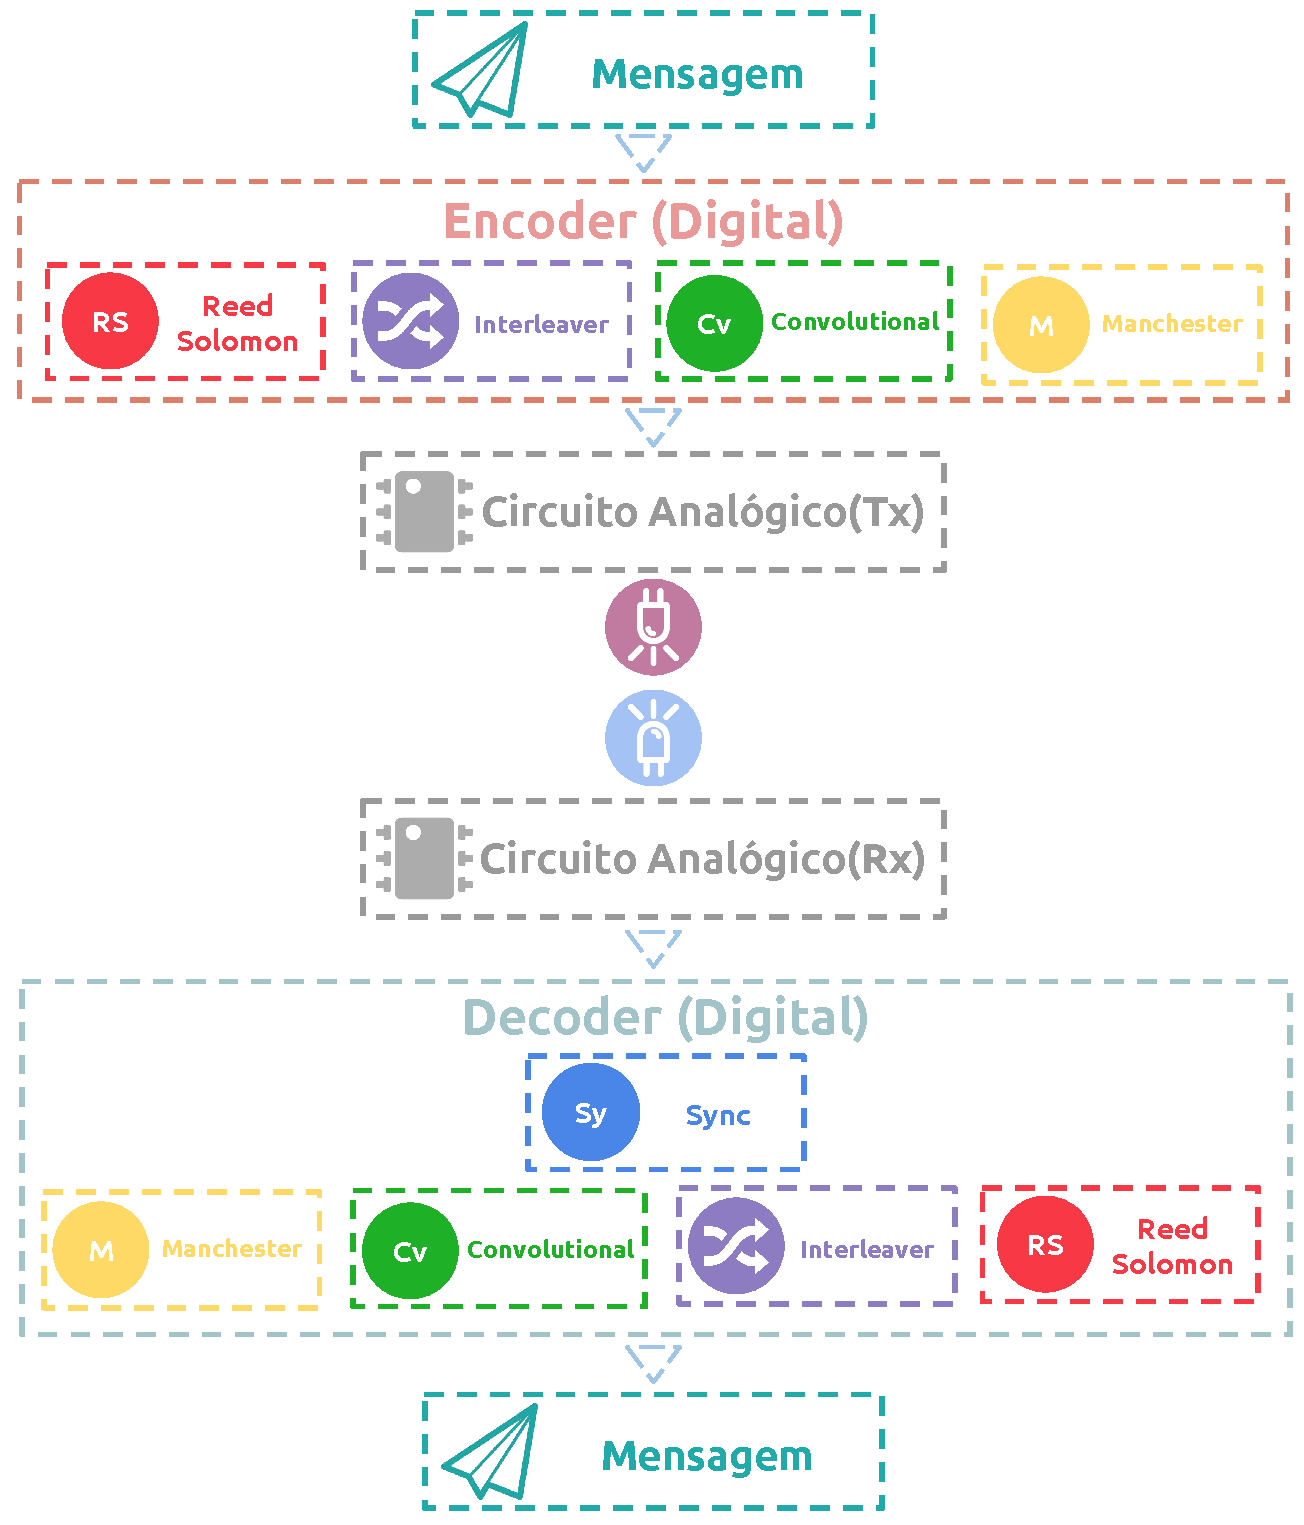
\includegraphics[width=1\textwidth]{Arquitetura.pdf}
		\legend{Fonte: Autores.}
	\end{figure}
	
	A seguir, explicam-se os componentes indicados dentro de Encoder e Decoder, que em conjunto sintetizam todos os circuitos digitais do estudo. Explicitar-se-ão as decisões mais importantes de projeto e a forma pela qual se integraram e se testaram os dois módulos.

	
	\subsection{Codificador Reed Solomon}
	
	Conforme apontado no capítulo de Metodologia, a arquitetura do codificador Reed Solomon foi construída para um código (15, 7), portanto contando com 8 registradores em série. Os multiplicadores foram feitos com uma tabela,  que recebe duas entradas e retorna uma saída, de maneira a simplificar o trabalho de fazer uma função utilizando lógica combinatória. Já os somadores são equivalentes à função de OU exclusivo, ou XOR, com duas entradas e uma saída de 4 bits cada - ou seja, um símbolo. Além destes, os módulos básicos ainda compreendem um multiplexador, que seleciona um entre dois símbolos. A arquitetura desenvolvida pode ser observada na \autoref{RS_encoder_logic}.
	
	O comportamento de codificação de uma mensagem pode ser exemplificado pela \autoref{simula_rs_encoder}, onde se observa a entrada de uma mensagem de 7 símbolos e a saída de um bloco de 15 símbolos, sendo 8 de paridade.
	
	\begin{figure}[h]
		\caption{\label{simula_rs_encoder}Simulação de codificação do codificador Reed Solomon.}
		\centering
		\includegraphics[width=1.0\textwidth, trim={0 0 5cm 0}]{RS/Sim_encoder}
		\legend{}
	\end{figure}
	
	\subsection{\textit{Interleaver}}

	O módulo do Interleaver é composto por três componentes principais: (i) a memória, (ii) a unidade de controle do cabeçalho e (iii) a unidade de controle do payload.

	\subsection{Memória}
	
	Para realizar o processo de entrelaçamento, é necessário que o \textit{Interleaver} guarde a mensagem inteira dentro de uma memória, para manipular sua ordem de disposição. 
	
	Deve-se observar, no entanto, que o tamanho da mensagem a ser guardado é maior que apenas o tamanho máximo do payload da PHY I (1023 \textit{bytes}). Isso acontece pois o módulo anterior ao \textit{Interleaver} - o Codificador Reed Solomon - transforma cada 28 bits de mensagem em 60 bits (Reed Solomon (15,7)). A mensagem com paridade adicionada ao fim tem portanto 2191 \textit{bytes}. Além disso, ainda deve ser considerado o cabeçalho, sua paridade e seu padding (4 + 3 + 8 \textit{bytes}). Portanto o Interleaver deve ser capaz de guardar 2206 \textit{bytes}.
	
	A princípio, é possível realizar esse armazenamento de três formas na FPGA: (i) criando vetores dentro de um arquivo .vhd, (ii) utilizando uma memória externa a FPGA e (iii) utilizando uma memória interna da FPGA. A primeira solução ocupa muito espaço disponível nas unidades lógicas do chip. A segunda proposta requer uma memória acoplada à placa de desenvolvimento utilizada, restringindo a gama de placas possíveis. A terceira e última opção é a mais adequada, pois a arquitetura da FPGA utilizada (EP4) possui memória auxiliar incorporada na FPGA.
	
	Para implementar a memória, foi utilizado o componente RAM de duas portas do Catálogo IP (Intellectual Property) do programa Altera Quartus. De forma que a capacidade de memória seja no mínimo 2206 \textit{bytes}, foi instanciada uma de 4096 \textit{bytes}, pois devem ser potências de 2.

	\subsection{Unidade de controle do cabeçalho}\label{section:interleaver-header-control}
	
	O propósito deste módulo é receber os dados do Codificador Reed Solomon, gravá-los na memória interna e depois enviá-los de forma entrelaçada. A abordagem tomada pelo projeto foi gravar esses dados em ordem entrelaçada, para que a leitura seja feita apenas varrendo os endereços da memória em ordem crescente. A \autoref{figure:interleaver-order} ilustra o algoritmo desenvolvido para escolher os endereços entrelaçados. Ele foi implementado em Javascript para melhor visualização da ordem certa de gravação.
	
	\begin{figure}[h]
		\caption{\label{figure:interleaver-order}Ordem do algoritmo entrelaçador para gravar a memória.}
		\centering
		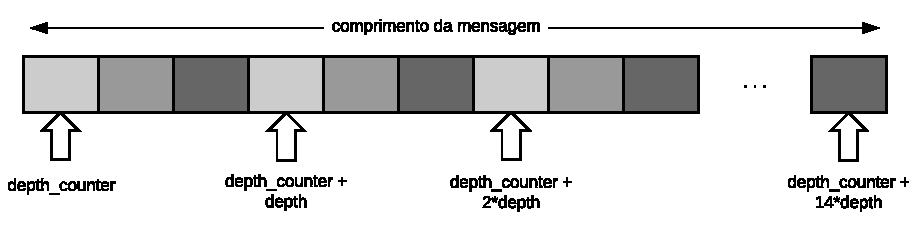
\includegraphics[width=0.9\textwidth]{interleaver/order.pdf}
		\legend{Fonte: Autores.}
	\end{figure}
	
	Em VHDL, a solução é composta por três componentes: (i) contador de endereços, (ii) contador de profundidade e (iii) contador de saída. Eles estão integrados com a memória na \autoref{figure:interleaver-schematics}.
		
	\begin{figure}[h]
		\caption{\label{figure:interleaver-schematics}Diagrama esquemático do \textit{Interleaver}, com unidade de controle e memória. Os sinais azuis representam entradas para melhor visualização.}
		\centering
		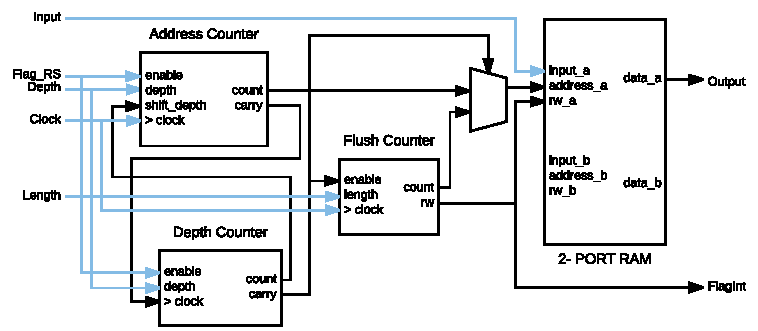
\includegraphics[width=1\textwidth]{interleaver/schematics.pdf}
		\legend{Fonte: Autores.}
	\end{figure}

	\paragraph{Contador de endereços}
	Responsável por selecionar endereços para a etapa de gravação da memória. Recebe 
	
	\paragraph{Contador de profundidade}
	
	\paragraph{Contador de saída}
	
	\begin{figure}[h]
		\caption{\label{figure:interleaver-flow}Diagrama esquemático do fluxo de dados do \textit{Interleaver}.}
		\centering
		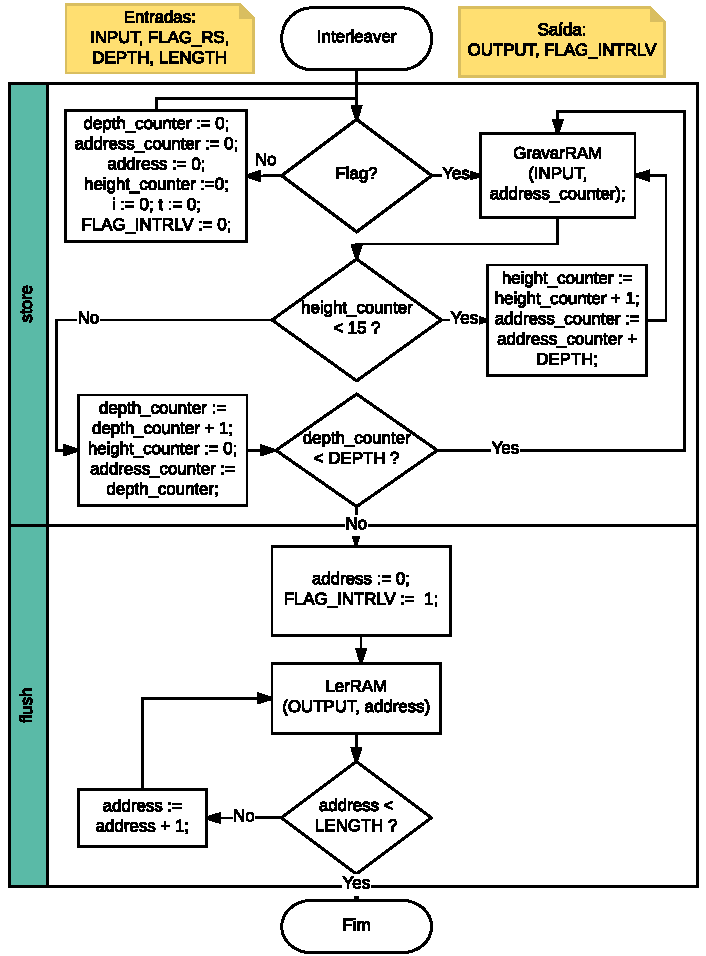
\includegraphics[width=1\textwidth]{interleaver/flow.pdf}
		\legend{Fonte: Autores.}
	\end{figure}
	
	\subsubsection{Unidade de controle do \textit{payload}}
	
	O comportamento da unidade de controle do \textit{payload} é análoga a explicada anteriormente (\autoref{section:interleaver-header-control}). Entretanto, é necessário que eles funcionem de forma coordenada, de acordo com o recebimento do cabeçalho e em seguida dos dados.
	
	\subsection{Codificador Convolucional}	
	
	O convolutional encoder foi implementado a partir de seis registradores representando a janela deslizante mencionada na metodologia e xor dos valores dos geradores polinomiais.
	Vale mencionar que existe um tratamento específico dos dados que saem do interleaver antes de entrar no convolutional encoder que consiste em dois módulos. Um módulo lida com o fato de que o interleaver tem saída de palavra por palavra, ou seja, de quatro em quatro bits e a entrada do convolutional encoder deve ser bit por bit. Ele transforma os dados de paralelos para seriais.
	O outro módulo insere uma cadeia de 6 bits zeros entre o header e o interleaver. Garantindo que o estado inicial conhecido seja “000000” para os dados serem posteriormente decodificados. Esse módulo conta as 30 (tamanho do header) primeiras palavras recebidas. Após atingir o fim do header a entrada começa a passar por um registrador de deslocamento de 6 bits inicialmente zerado.
	
	Puncture:
	
	Para realizar o puncture de $\frac{1}{4}$ o valor A é mantido pelo tempo equivalente a dois clocks do próximo módulo e o valor de B por mais dois clocks. Seguindo o que foi especificado na metodologia.
	
	\subsection{Codificador Manchester}
	
	A arquitetura da codificação de Manchester segue o mesmo modelo explicado na Metologia. Duas entradas: clock e mensagem, recebem a operação lógica XOR e retornam o código.
	
	
	\subsection{\textit{Sync}}
	
	Módulo que sincroniza o \textit{clock} do transmissor com o do receptor, para que os dados recebidos sejam os mesmos que os enviados. 
	
	Inicialmente foi utilizado uma propriedade intelectual da Altera chamada PLL (\textit{Phase-Locked Loop}). Um estudo mais detalhado demonstrou que sua entrada recebe apenas sinais de ordem de grandeza de MHz. É portanto incompatível com a frequência definida pela camada PHY I.
	
	O trabalho propõe uma solução para esse problema desenvolvida pelos próprios autores, e é dividida em três módulos: \textit{oversampling}, decisor de limite de tempo, detector de FLP e gerador de \textit{clock}. O diagrama abaixo (\autoref{figure:sync-schematics}) ilustra a conexão entre esses módulos.
	\begin{figure}[h]
		\caption{\label{figure:sync-schematics}Diagrama esquemático do \textit{Sync}.}
		\centering
		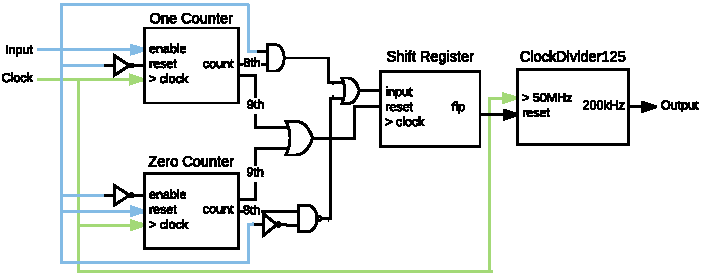
\includegraphics[width=1\textwidth]{sync/schematics.pdf}
		\legend{Fonte: Autores.}
	\end{figure}
	
	\subsubsection{\textit{Oversampling}}
	Componente que realiza a verificação do tempo de permanência do sinal para cada \textit{bit}. Possui dois contadores, um para o sinal lógico zero e outro para um. O próprio sinal de entrada habilita (\textit{enable}) o contador de zeros quando está em \textit{high}, e analogamente o contador de uns quando está em \textit{low}. O funcionamento do sinal de \textit{reset} é inverso ao de enable aos dois contadores. Portanto o módulo contador de zeros conta por quantos clocks de 50MHz a entrada ficou em zero. Caso a entrada seja um, o contador zera e ele é desabilitado. Analogamente para o módulo contador de uns, que conta por quantos clocks a entrada ficou em um, zerando.

	\subsubsection{Decisão de Limite de Tempo}
	Esse subsistema decide se o sinal analisado pelo módulo de \textit{Oversampling} possui pelo menos 250 amostras iguais (zeros ou uns). Ele parte do princípio que a entrada será uma onda quadrada de período 250 $\mu$s - garantido pelo envio do FLP -, não possuindo dois uns nem dois zeros seguidos.
	
	Com intuito de facilitar a sincronização, o decisor de limite de tempo verifica se o \textit{Oversampling} está dentro de um intervalo de 128 a 255 ciclos. Esse processo ocorre verificando apenas os bits mais significativos do contador. Caso o oitavo \textit{bit} seja um, significa que o módulo anterior contou pelo menos até 128, caracterizando um possível um ou zero. Verificando o nono \textit{bit} é possível concluir se ele não excedeu o tempo de permanência no mesmo \textit{bit} (além de 255). 
	
	Para o módulo sincronizador, dois uns ou dois zeros seguidos fogem da norma, portanto tais mensagens são descartadas.
	
	\subsubsection{Detector de FLP}
	A detecção de FLP é realizada com com um registrador de deslocamento de 200 \textit{bits}. Se pelo menos 200 bits recebidos preenchem o registrador com zeros e uns alternados, o móduto gera um sinal lógico um para o gerador de clock.
	
	O registrador é reiniciado quando o nono \textit{bit} do Decisor de limite de tempo é um, pois caracteriza um FLP inválido. Enquanto apenas o oitavo \textit{bit} for detectado, o registrador grava o valor e desloca seus valores à direita.
	\subsubsection{Gerador de \textit{clock}}
	Módulo que gera um \textit{clock} de 200kHz estável para o decodificador inteiro. Utiliza um divisor de frequência do \textit{clock} interno da FPGA.
	
	Quando recebe o sinal de detecção de FLP, reajusta seu clock de 200kHz forma que a borda de subida fique no centro do \textit{bit} de entrada. Essa característica do gerador de clock protege o decodificador do fenômeno de \textit{clock drift}, ou da perda de sincronia entre os clocks devido ao comprimento da mensagem.
	\subsection{Decodificador Manchester}
	
	O decodificador funciona, conforme explicado anteriormente, de acordo com a \autoref{tabela_cod_manchester}.
	
	Neste projeto, o decodificador de Manchester é inicializado quando o TDP~TDPTDP~TDP é identificado. Seu circuito foi desenvolvido com uma máquina de estados que tem estado inicial S0. Essa máquina funciona de modo que quando existe uma transição de 0 para 1, a saída é um bit 0 e quando a transição é de 1 para 0, a saída é um bit 1 para 0. Isso é demonstrado na figura \autoref{figure:manchester-decoder-flow}. 
		
	\begin{figure}[h]
		\caption{\label{figure:manchester-decoder-flow}Visão de máquina de estados do decodificador Manchester.}
		\centering
		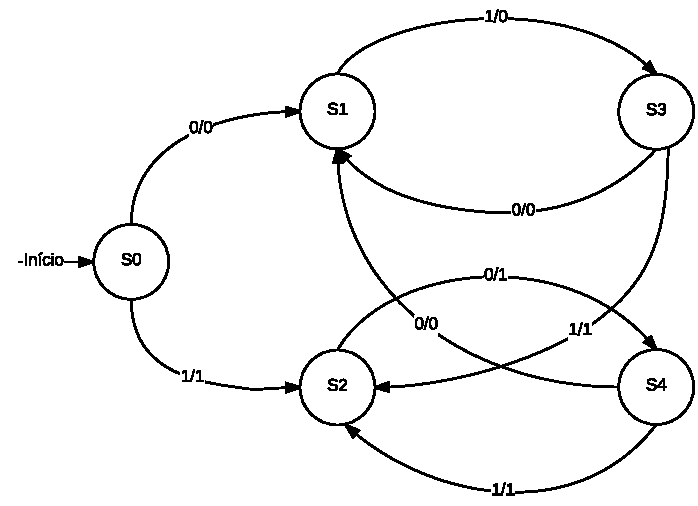
\includegraphics[width=0.6\textheight]{manchester/decoder-flow.pdf}
		\legend{Fonte: Autores.}
	\end{figure}
	
	
	\subsection{Decodificador Viterbi Fangled}
	
	Os dados são transformados de seriais paralelos de 4 em 4 para encaixarem com a entrada do fangled viterbi decoder
	Para decodificação dos dados fornecidos pelo codificador convolucional foi utilizado o fangled  viterbi decoder. Ele é uma versão simplificada do viterbi decoder. Utiliza menos memória, e menos processamento, é mais veloz porém tem capacidade de detecção e correção de erro muito menor. A capacidade de correção de erro é de um bit a cada quatro dado que o puncture do convolutional é de $\frac{1}{4}$.
	Branch Metrics: A entrada é composta por AABB. Calcula-se a distância entre o primeiro A com o primeiro B e todas as possíveis combinações de bits (00, 01, 10, 11). A distância é calculada do mesmo modo para o segundo A e o segundo B recebidos. Isso foi feito a partir da operação xor entre a entrada e as combinações. As distâncias de uma mesma combinação de bits é posteriormente somada.
	Trellis Table: Dado o estado atual, é um look up table que os dois valores possíveis de entrada pro viterbi. Uma delas é caso o bit que foi codificado fosse um e o outro caso é se ele fosse zero.
	Path Metrics: O path metrics recebe a informação de quais as duas possíveis entradas do Trellis Table e quais as distâncias do branch metrics. Com esses dados o path metrics identifica qual o bit mais provável de ter sido codificado. Definindo, assim, qual o próximo estado e a saída do viterbi decoder. 
	O valor do próximo estado é armazenado para ser posteriormente utilizado pelo Trellis Table.
	Caso as distâncias a serem consideradas forem iguais, o valor da saída é escolhido como sendo zero e o próximo estado é definido de acordo com isso. Segue-se a ideia do fangled viterbi decoder que escolhe uma saída, e consequentemente o próximo estado, ao acaso. 
	
	
	\subsection{Decodificador Reed Solomon}
	
	A arquitetura do decodificador segue o diagrama funcional da figura X do capítulo de Metologia. Desta forma, o desenvolvimento pode ser separado em quatro partes principais, apresentadas a seguir.
	
	\subsubsection{Cálculo das Síndromes}
	
	O cálculo das síndromes é feito de forma iterativa, durando tantos ciclos quanto forem os símbolos da mensagem. O cálculo de cada síndrome é independente dos cálculos das demais, e depende apenas dos símbolos de entrada e de cada uma das raízes do polinômio codificador, de alpha0 a alpha7 neste caso. O arranjo dos componentes pode se exemplificar através da arquitetura do módulo, representada na \autoref{fig_sindrome_arq} nos Anexos.

	Os elementos indicados por "static" são constantes, guardando os valores dos símbolos de cada umas raízes citadas. Estes valores são enviados para multiplicadores de GF(16), representados por "gfmult". Como pode-se observar, o cálculo é iterativo e portanto os multiplicadores recebem também o valor dos registradores que são representados por "register4b". Os somadores de Campos de Galois são representados por "gfsum".
	
	A simulação a seguir representa o caso em que existem erros na mensagem codificada, o que é indicado por síndromes diferentes de 0000.
	
	\begin{figure}[!htb]
		\caption{\label{fig_sindrome_sim}Simulação do cálculo das síndromes.}
		\centering %%trim={<left> <lower> <right> <upper>}
		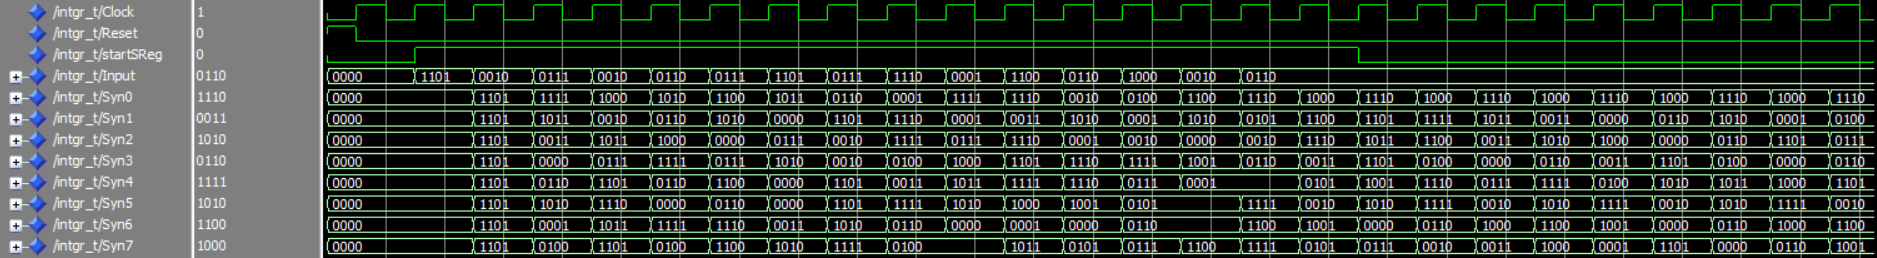
\includegraphics[width=1\textwidth, trim = {0 0 15cm 0}]{RS/Sim_sindrome.PNG}
		\legend{}
	\end{figure}

	\subsubsection{Módulo de Berlekamp-Massey}
	
	O módulo de Berlekamp-Massey foi implementado de forma a primeiramente calcular as localizações dos erros, ou seja, os coeficientes do polinômio localizador de erros, representados por Lamba, e guardados em registradores, para o posterior cálculo dos valores dos erros. Os valores de erros são calculados então, com as síndromes e localizações de erro.
	
	As síndromes são enviadas sequencialmente para o módulo de Berlekamp-Massey a cada ciclo de clock. A atualização do polinômio localizador, representado pela seção X do diagrama, ocorre quando ele não possibilitar gerar uma síndrome específica. Nesse caso, são feitos os cálculos no módulo inversor, com a atualização do polinômio no próximo ciclo. Esse processo é exemplificado pela \autoref{fig_berlekamp_sim}.
	
	\begin{figure}[!htb]
		\caption{\label{fig_berlekamp_sim}Simulação do módulo de Berlekamp-Massey.}
		\centering
		\includegraphics[width=1\textwidth, trim = {0 0 14cm 0}]{RS/Sim_berlekamp.PNG}
		\legend{}
	\end{figure}
	
	Uma vez calculados os valores dos coeficientes do polinômio localizador, equivalentes a Lambda na simulação, é necessário calcular os coeficientes do polinômio de valor dos erros. Novamente, as síndromes são enviadas sequencialmente para o circuito. O novo cálculo ocorre com as síndromes e o polinômio localizador de erros. O resultado são os coeficientes do polinômio de valores de erro, representados por Omega na simulação, obtidos em sequência em cada ciclo de clock. 
	
	O componente de Berlekamp-Massey possui um circuito de controle próprio. Por ele é recebido um sinal de início de cálculo, vindo do controlador do estágio anterior, de cálculo de síndromes. Sendo assim, ele deve manipular registradores, para, por exemplo, registrar os valores de Lambda e Omega para cálculo posterior, no módulo seguinte.
	
	\subsubsection{Módulos de Busca de Chien e Forney}
	
	O módulo de busca de Chien é na verdade composto por dois módulos: busca de localização e de valores dos erros. Ambos trabalham paralelamente e têm como entrada os coeficientes $\Lambda$ e $\Omega$. 
	
	Pode-se observar que ambos funcionam com cálculo incremental. A cada ciclo, o valor de registradores é atualizado com o uso das raízes do polinômio codificador e dos coeficientes já apontados. As suas saídas vão diretamente para o módulo de Forney, uma delas indicando se deve-se corrigir o símbolo de mensagem, e outra indicando qual o valor da correção, que somado ao valor da mensagem corrigi quaisquer erros. É importante apontar que caso haja mais do que 4 símbolos com erros, nenhuma correção será feita, o que configura a condição para descarte do bloco recebido. É possível neste circuito observar esse processo com a identificação de síndromes diferentes de zero, com o sinal "errorsyndrome" na \autoref{fig_forney_sim}. Considerando que o sinal está na posição alta, significa que pelo menos um bit de alguma das síndromes é diferente de 0, e portanto a mensagem deve ser corrigida. 
	
	\begin{figure}[!htb]
		\caption{\label{fig_forney_sim}Simulação do módulo de Forney.}
		\centering%%trim={<left> <lower> <right> <upper>}
		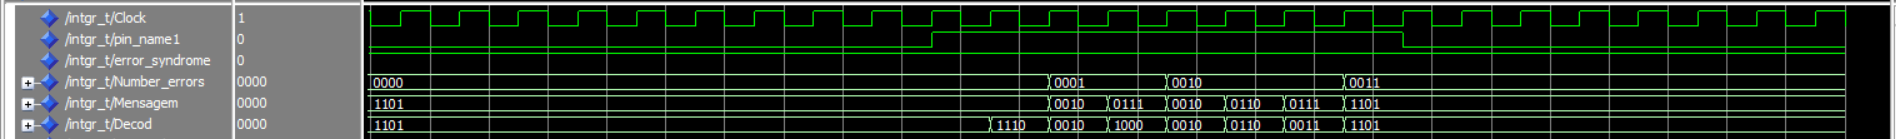
\includegraphics[width=1\textwidth, trim={0 0 15cm 0}]{RS/Sim_forney.PNG}
		\legend{}
	\end{figure}
	
	Por outro lado, caso haja mais de 4 símbolos com erro, nenhuma correção será feita, portanto contabiliza-se o número de correções feitas até então. Se for identificado um erro com as síndromes e não for contada nenhuma correção no módulo de Forney, temos duas condições suficientes para afirmar que o bloco deve ser descartado e este não pode ser corrigido através do método de Reed Solomon. No exemplo anterior, o número de erros corrigidos é inferior a 5, portanto a mensagem final está correta e pode sair da camada física PHY I. Caso a mensagem seja descartada, é necessário que se envie novamente pelo transmissor.	
	

	
	% ---
	\section{Hardware analógico}
	% ---
	A seção abaixo discorrerá sobre a aplicação dos métodos estudados nos capítulos anteriores para Hardware analógico.
	Antes de iniciar a execução do trabalho, foram estabelecidas algumas decisões de projeto:
	
	* formato de lista *
	Única fonte de alimentação de 5V.
	Implementação de um circuito apenas para a camada PHY I da norma, fixando a frequência de operação a 200kHz.
	
	. . .
	
	\subsection{Transmissor}
	
	\subsubsection{Conversor Digital-Analógico}
	Com os estudos feitos na \autoref{section:dac}, é possível especificar os requisitos reais para o transistor de potência:

	\begin{itemize}
		\item Tensão de base/\textit{gate} compatível com 3.3V;
		\item Corrente de saída compatível com LED de alta potência, no mínimo 750mA;
		\item Resposta de base/\textit{gate} a $V_{on(FPGA)}$ de no máximo 1us;
	\end{itemize}
	
	Alguns dos parâmetros são decisões de projeto, como a utilização de níveis TTL (Transistor Transistor Logic) para chaveamento do transistor (3.3V ou 5V), e outros são requisitos da norma IEEE, como frequência de operação a 200kHz. Especialmente no segundo caso, é importante escolher um transistor com $T_{rise}$ e $T_{fall}$ de no mínimo 10-100 vezes menor que o período da onda transmitida - no caso $5\mu$$s/100 = 50ns$. Se o transistor não chavear rápido suficiente, é possível que a onda seja alterada. Em alguns casos é possível que fique semelhante a uma onda "dente de serra".
	
	O componente escolhido foi um MOSFET de Potência, mais especificamente o IRLZ14, pois é um transistor de nível lógico e tem o \textit{gate} compatível com voltagens de microcontrolador. 

	De acordo com função de transferência da \autoref{figure:transfer-carac-irlz14}, a VGS=3.3V é permitida uma corrente de dreno de 2A. A \textit{datasheet} também especifica parâmetros de resposta dinâmica do circuito, como seu $T_{rise}$, $T_{fall}$, que estão disponibilizados na \autoref{table:irlz14-timing}.
	
	\begin{figure}[h]
		\caption{\label{figure:transfer-carac-irlz14}Características de transferência do MOSFET de potência IRLZ14.}
		\centering
		\includegraphics[page=3, width=0.4\textwidth, trim={12cm 16.5cm 2.2cm 5cm}, clip]{circuits/irlz14.pdf}
		\legend{Fonte: \cite{datasheet-irlz14}}
	\end{figure}

	\begin{table}[h]
		\caption{Características Dinâmicas do MOSFET IRLZ14.}
		\centering
		\begin{tabular}{c c}
			\hline
			Parâmetro  & Valor  \\ \hline
			$T_{rise}$ & 110 ns \\
			$T_{fall}$ & 26 ns  \\ \hline
		\end{tabular}
		\label{table:irlz14-timing}
		\legend{Fonte: \cite{datasheet-irlz14}}
	\end{table}

	\subsubsection{Transmissão de Luz}
		
	Para realizar a transmissão de luz a distâncias de pelo menos um metro, será necessária a utilização de um LED de potência. Esse LED deverá atender a requisitos de altas frequência e resposta luminosa de acordo com seu chaveamento. Procurando satisfazer tais parâmetros, o componente escolhido foi o LUW W5-AM, fabricado pela OSRAM.

	Utilizando o circuito polarizador do LED da \autoref{figure:led-circuit}, é necessário calcular o valor da resistência de $R_{LIMIT}$. O LED permite no máximo 1000mA de corrente de polarização, mas não é desejável trabalhar na região limite de corrente, portanto o circuito será projetado para funcionar a 500mA. Como a voltagem de operação é de 5V, utilizando a Lei de Ohm:
	\begin{equation}
	R_{LIMIT} = 5V \cdot 500mA = 2.5\Omega
	\end{equation}
	
	\subsubsection{Versões Anteriores}
	
	Devido a falta de conhecimento do comportamento de transistores e da resposta de todos os componentes a frequência de 200kHz, foram projetados vários circuitos que não satisfaziam o formato de onda desejado. Abaixo são exemplificadas algumas versões implementadas, juntamente com os motivos de terem sido abandonadas.
	
	\paragraph{Filtro da Ponta de Prova}
	\begin{figure}[htb]
		\caption{\label{fig_transmitter_lify_circuit_fail0}Circuito de transmissão com filtro de ponta de prova.}
		\centering		%  trim={<left> <lower> <right> <upper>} 
		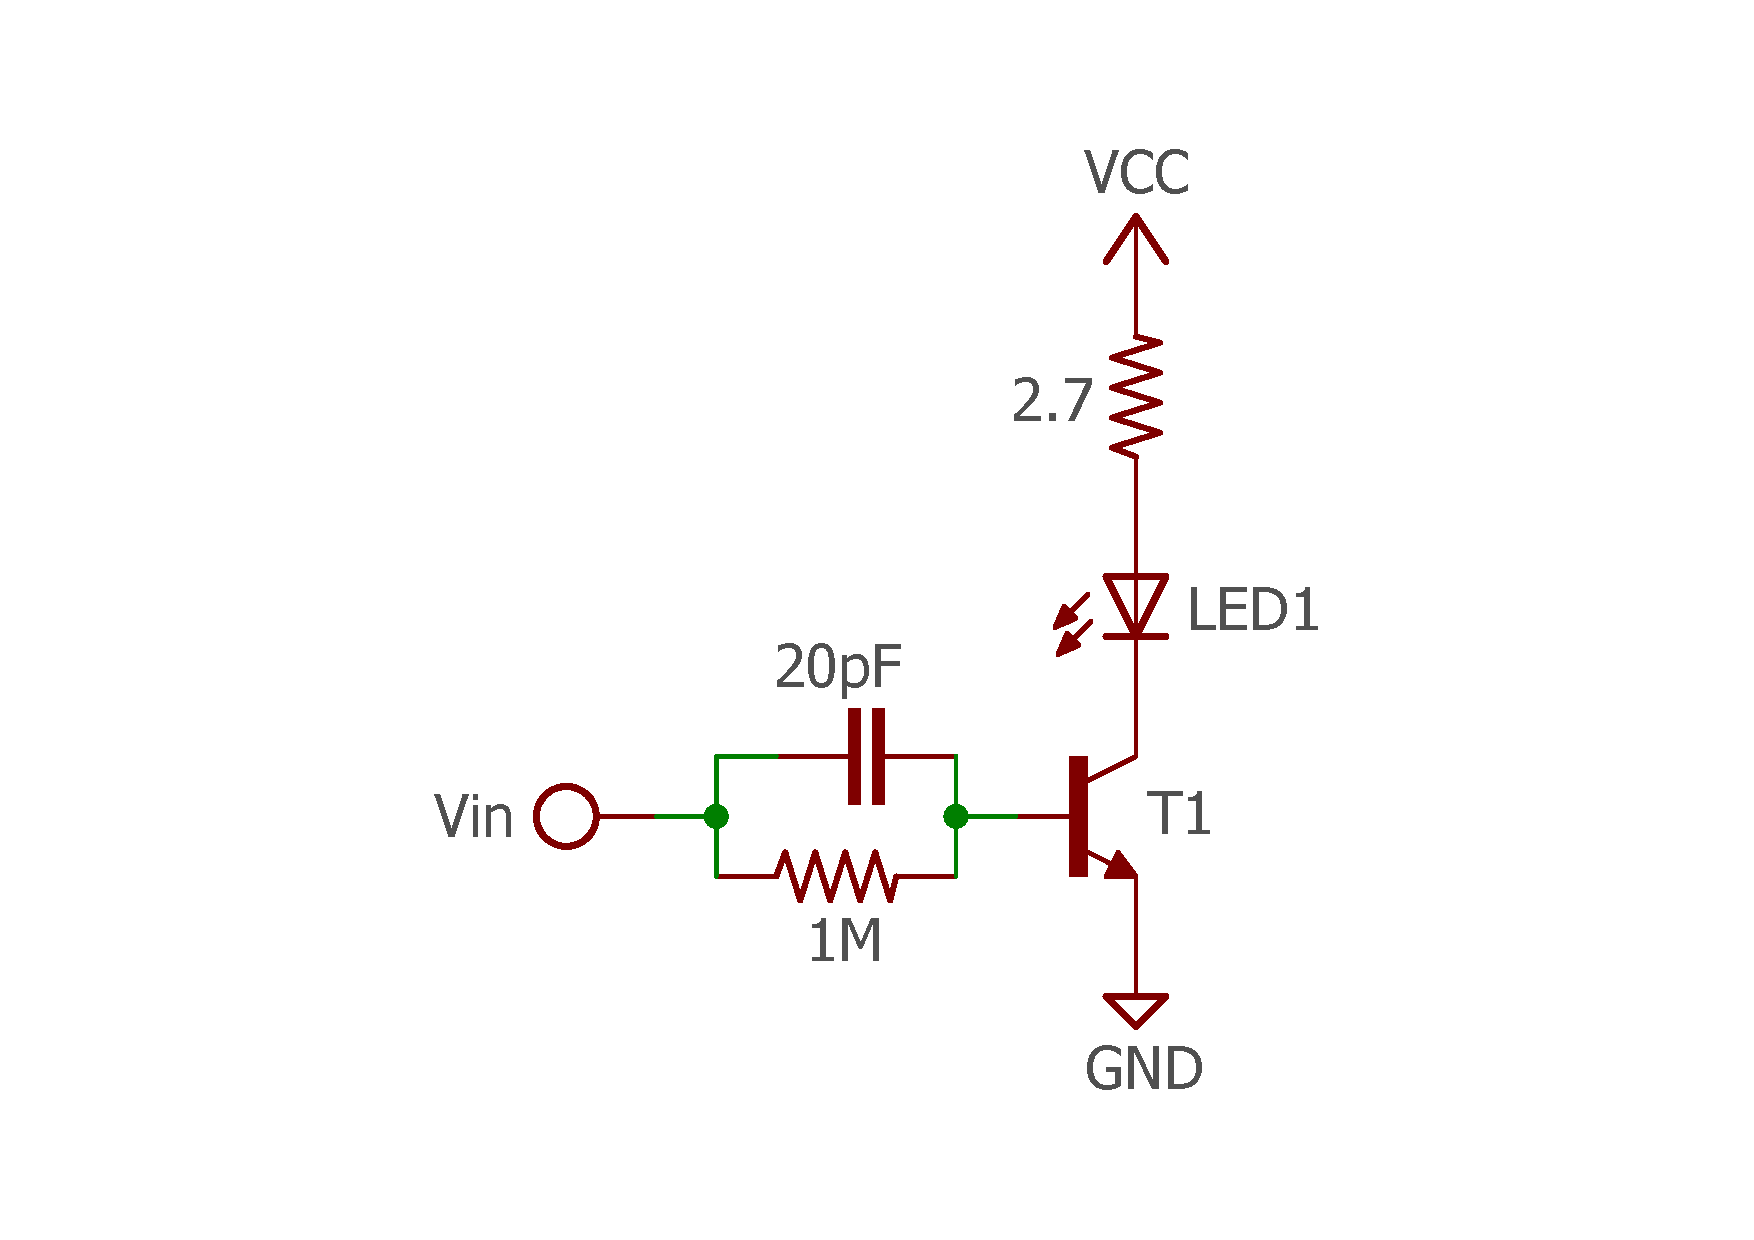
\includegraphics[width=0.5\textwidth, trim={2cm 1cm 2cm 2cm}, clip]{circuits/transmitter_fail0.pdf}
		\legend{Fonte: Autores.}
	\end{figure}
	O primeiro problema que o projeto do transmissor encontrou foi o comportamento de subamortecimento nos terminais do LED. Ele utiliza um circuito semelhante ao utilizado em pontas de provas para filtrar ruídos e é conectado em série com a entrada do transmissor, como visto na \autoref{fig_transmitter_lify_circuit_fail0}.
	\begin{figure}[htb]
		\caption{\label{fig_transmitter_lify_circuit_fail0_rl}Comportamento do circuito de transmissão com filtro de ponta de prova em série com a entrada. A onda azul é saída do gerador de funções enquanto a onda amarela é a tensão submetida ao LED. Observa-se o comportamento de subamortecimento em ambas.}
		\centering		%  trim={<left> <lower> <right> <upper>} 
		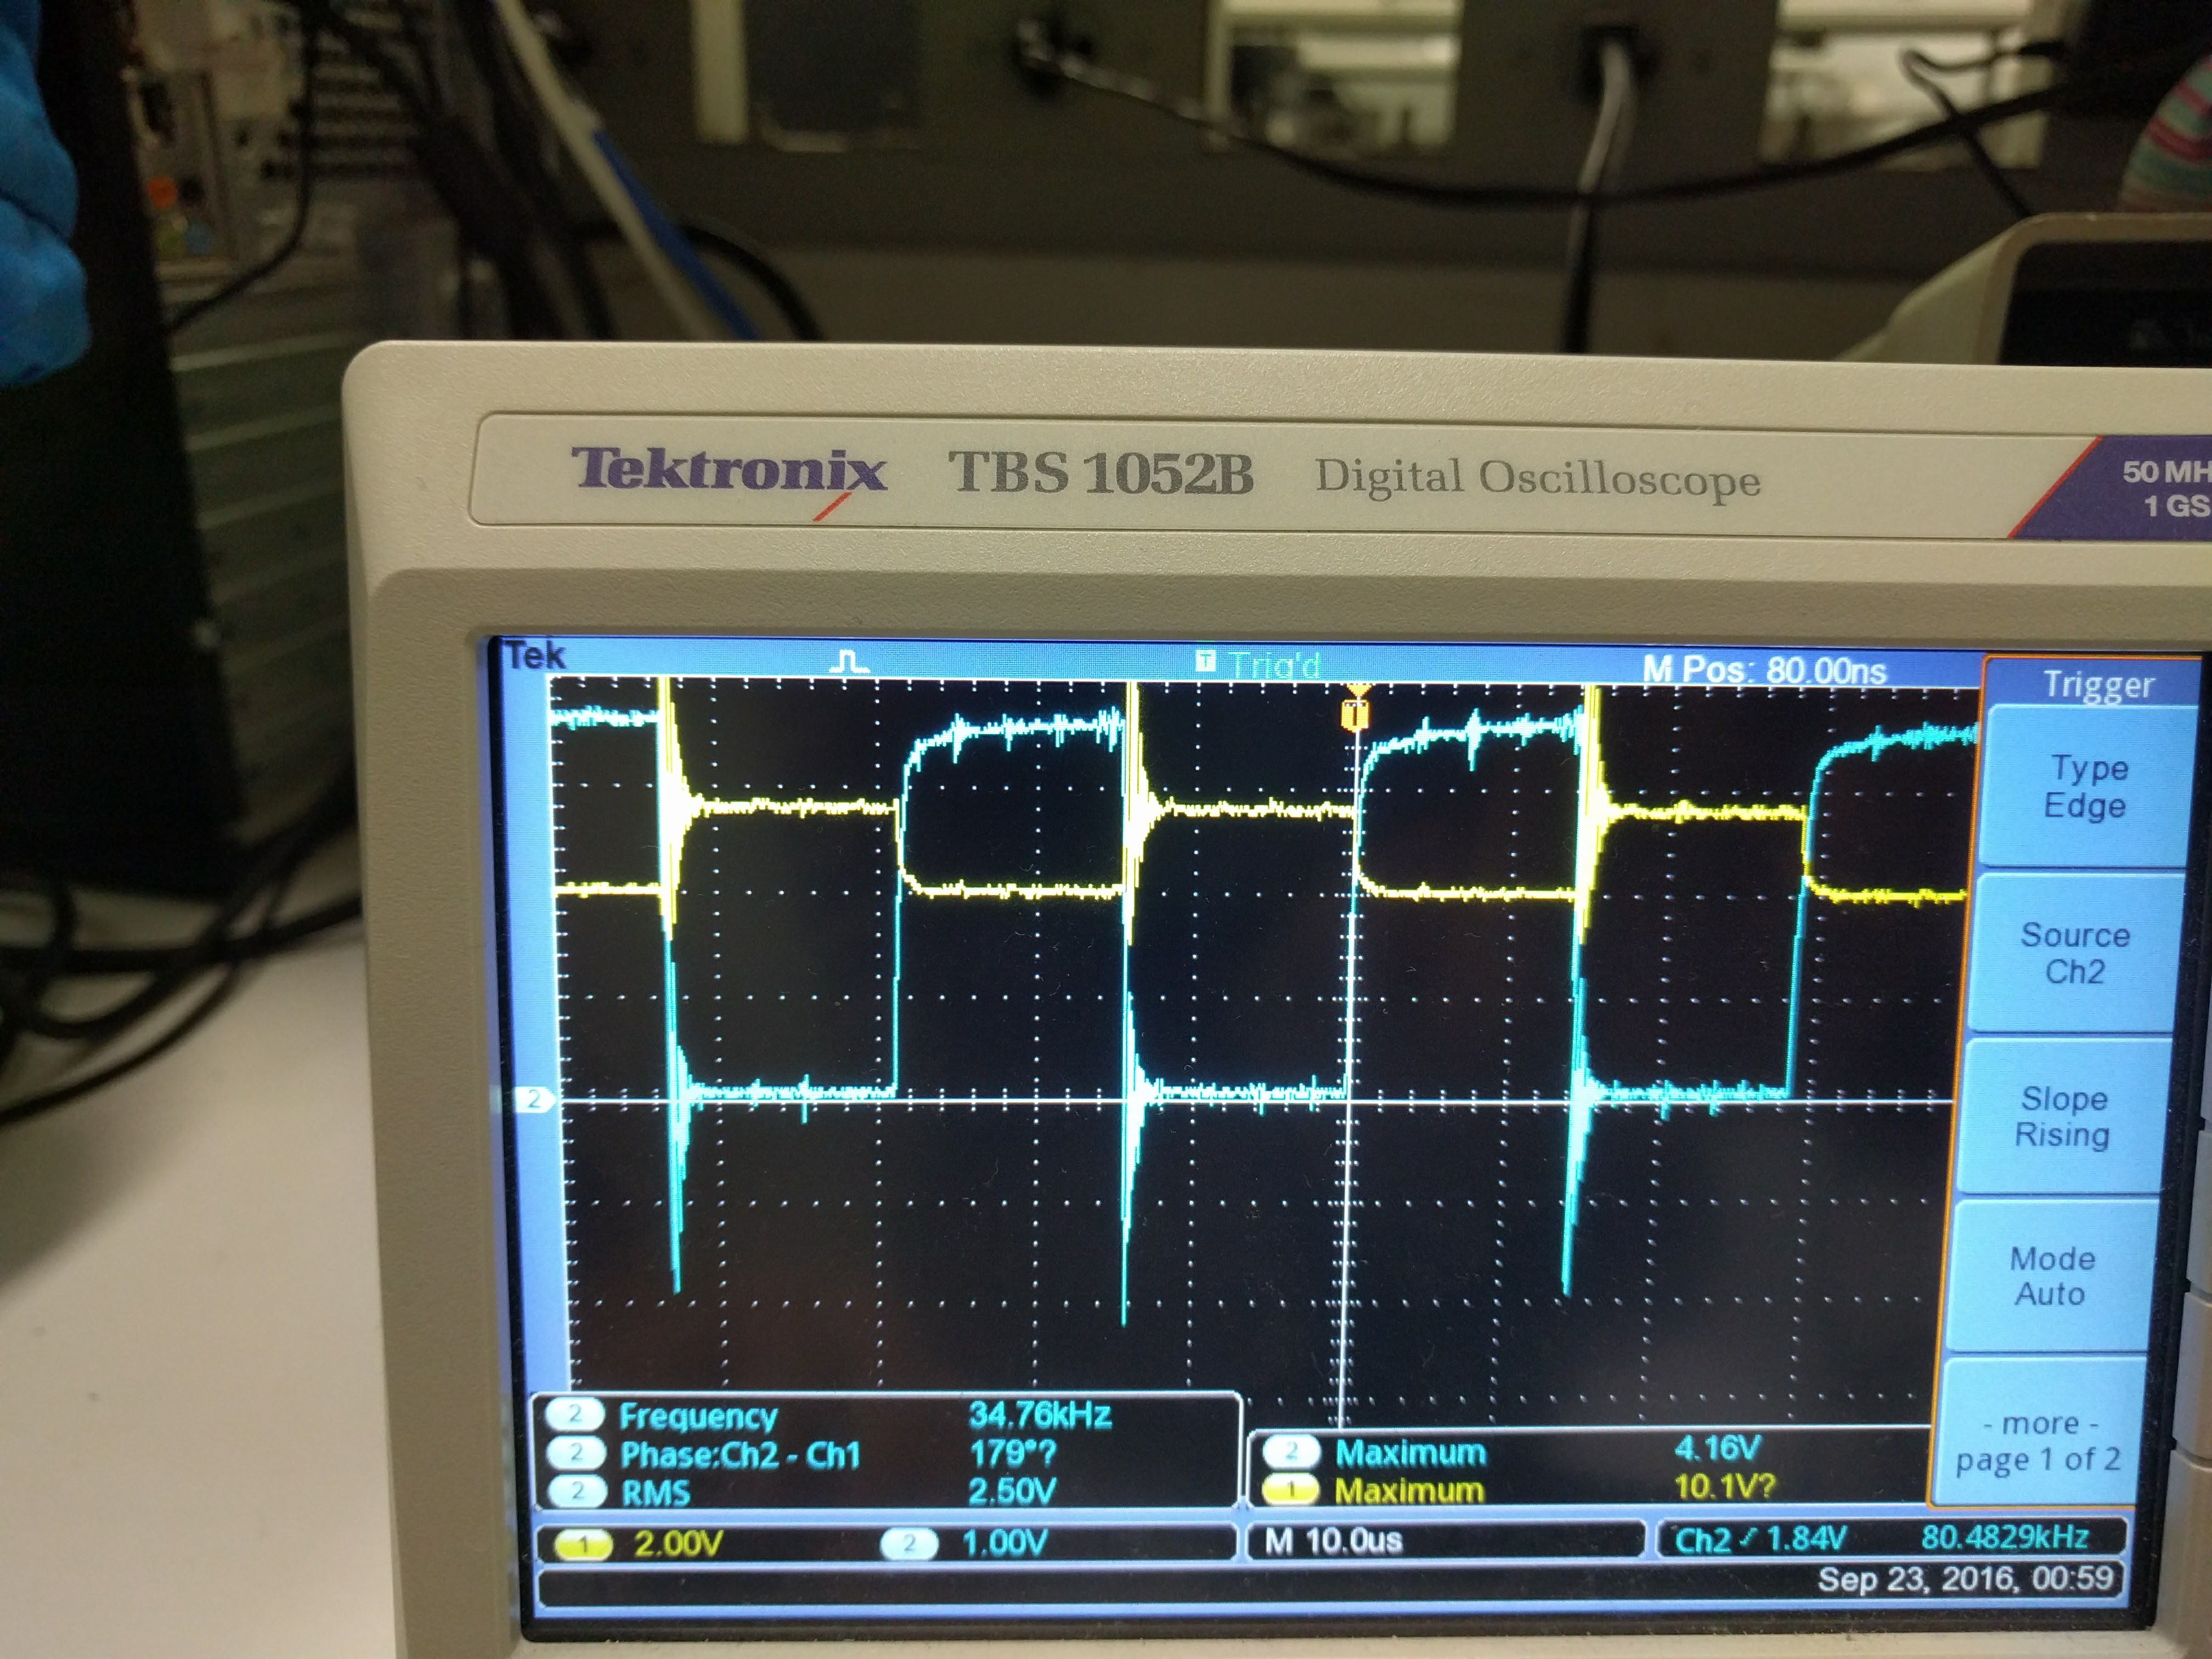
\includegraphics[width=0.5\textwidth, trim={30cm 0cm 2cm 40cm}, clip]{circuits/photos/TX_probe_result.jpg}
		\legend{Fonte: Autores.}
	\end{figure}

	A saída dessa implementação é mostrada na \autoref{fig_transmitter_lify_circuit_fail0_rl} e não foi satisfatória. O primeiro ponto a se notar é que a frequência de operação era baixa, no caso 80kHz - ainda 120kHz abaixo da especificação da velocidade da camada PHY I. Além dessa frequência a forma de onda se distorcia demais. O segundo ponto observado foi o fato de que houve uma resposta de subamortecimento tanto na entrada quanto na saída. Atribuiu-se esses efeitos a capacitâncias parasitas no LED e no transistor de potência.
	
	O transistor de potência possui capacitância devido a separação de suas placas. Seu valor é significativo e é até especificado na \textit{datasheet}. Para o IRLZ14, a capacitância de entrada é 400pF e de saída 170pF. Esses valores devem ser levados em conta ao polarizar tal componente. 

	No caso do LED, esse comportamento é mais complexo. A altas frequências, seu chaveamento cria um capacitor entre seus terminais, devido a sua arquitetura semicondutora. É possível observar esse comportamento capacitivo tanto em um LED de baixa potência quando de alta. Na prática, a tensão sob o LED não diminui acompanhando a tensão submetida a ele, e isso causa o comportamento indesejável visto, como os picos na onda amarela.
	
	A forma de onda gerada por esse circuito é muito boa, porém os picos de voltagem de até o dobro de $2 \cdot V_{CC} = 10V$ com certeza danificam os componentes. Essa versão foi descartada por esse motivo (como pode-se observar em no osciloscópio - \textbf{Maximum 10.1V}). 
	
	Em um teste unitário, foi observado o comportamento do chaveamento de um resistor $R_{L}$ a 200kHz, removendo completamente o LED do sistema. A saída observada era exatamente igual a entrada. Colocando um LED em série com o resistor adicionava o comportamento subamortecido, portanto conclui-se que a anomalia é atribuida ao LED.
	
	\paragraph{Aumento da Frequência}

	O aumento da frequência de operação a $f_{OP}$ = 200kHz causa um subamortecimento substancialmente maior. Observa-se na \autoref{fig_transmitter_lify_circuit_fail1_r1}, que provém de circuito sem o filtro da ponta de prova na \autoref{fig_transmitter_lify_circuit_fail1}.
	\begin{figure}[h!]
		\caption{\label{fig_transmitter_lify_circuit_fail1}Circuito de transmissão sem o filtro de ponta de prova.}
		\centering
		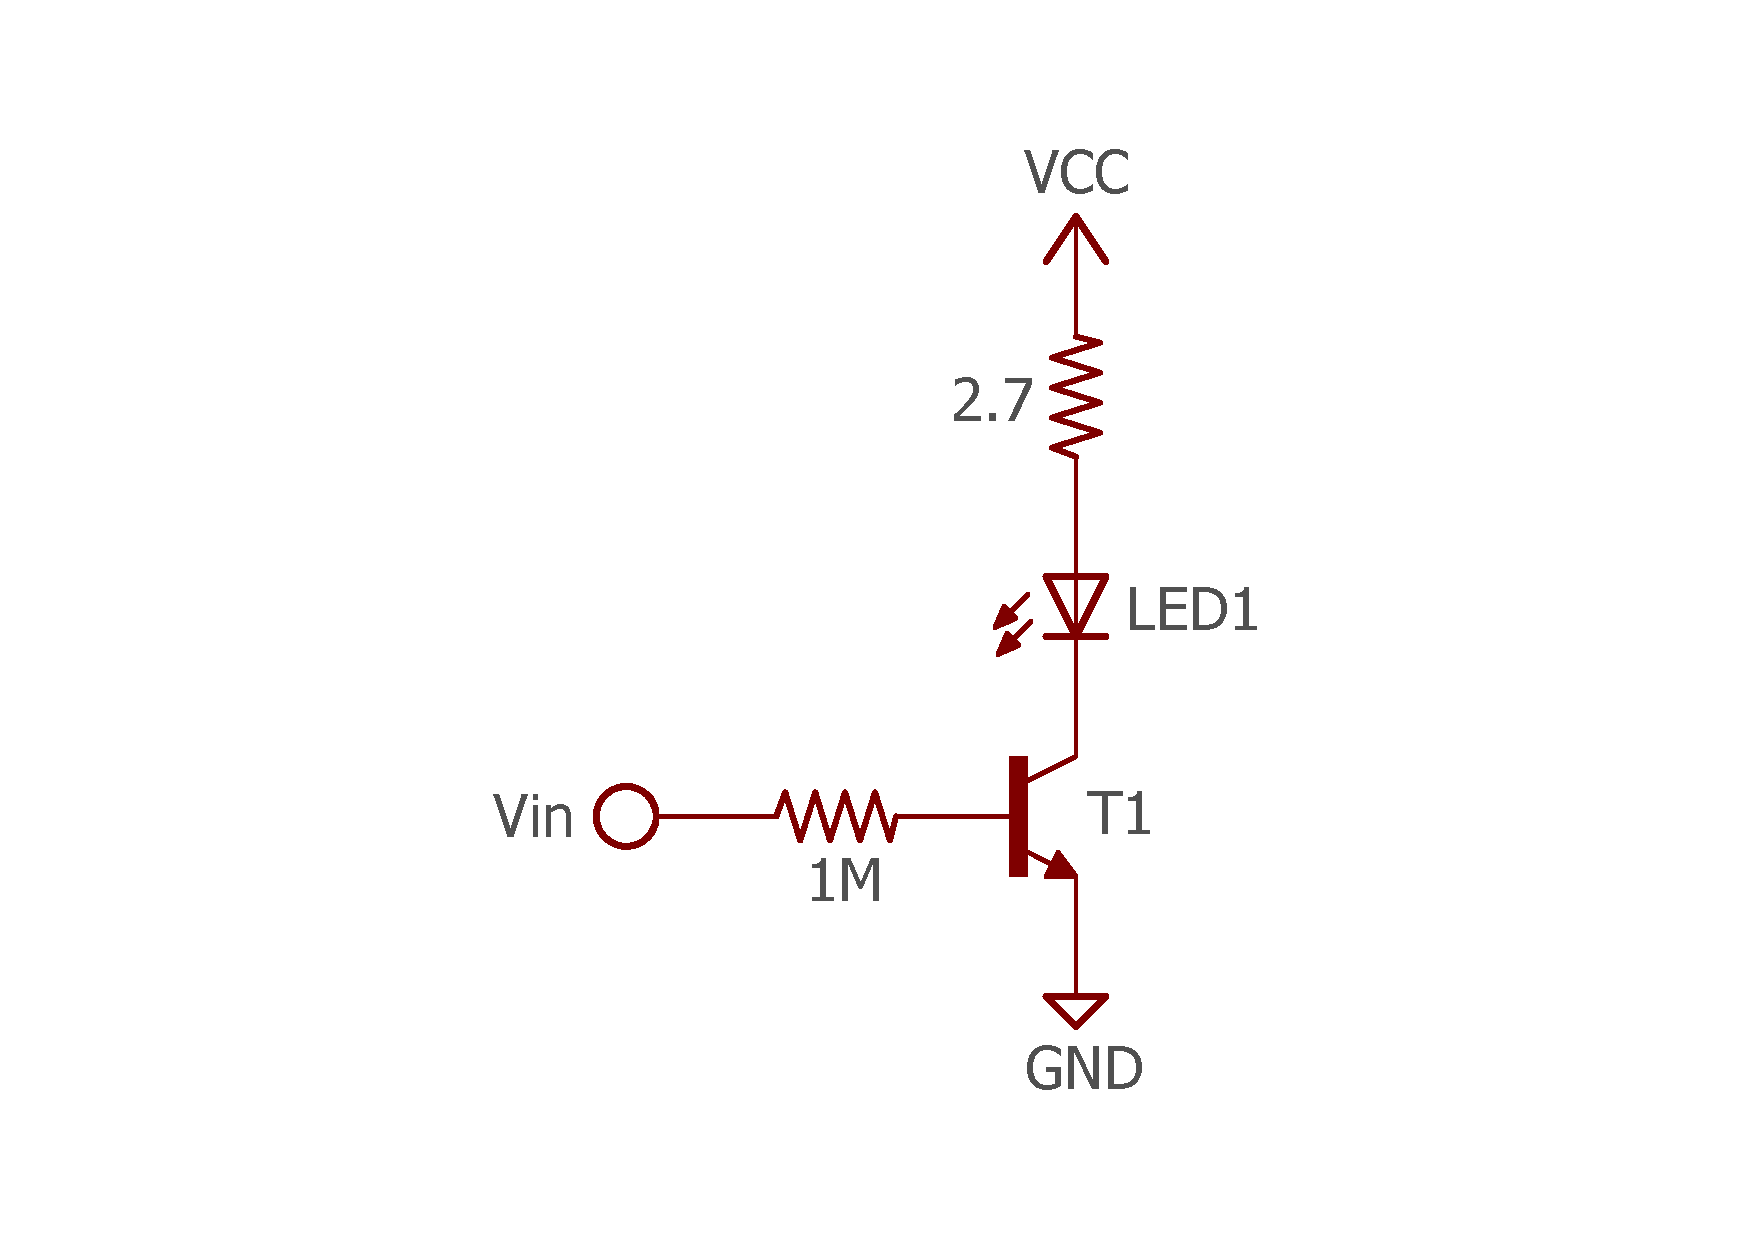
\includegraphics[width=0.5\textwidth, trim={2cm 2cm 2cm 2.3cm}, clip]{circuits/transmitter_fail1.pdf}
		\legend{Fonte: Autores.}
	\end{figure}
	\begin{figure}[h!]
		\caption{\label{fig_transmitter_lify_circuit_fail1_r1}Operação de circuito transmissor sem ponta de prova. A onda amarela representa voltagem no LED sem filtro de ponta de prova em frequências mais altas. O gerador de funções é medido e gera a forma de onda verde.}
		\centering
		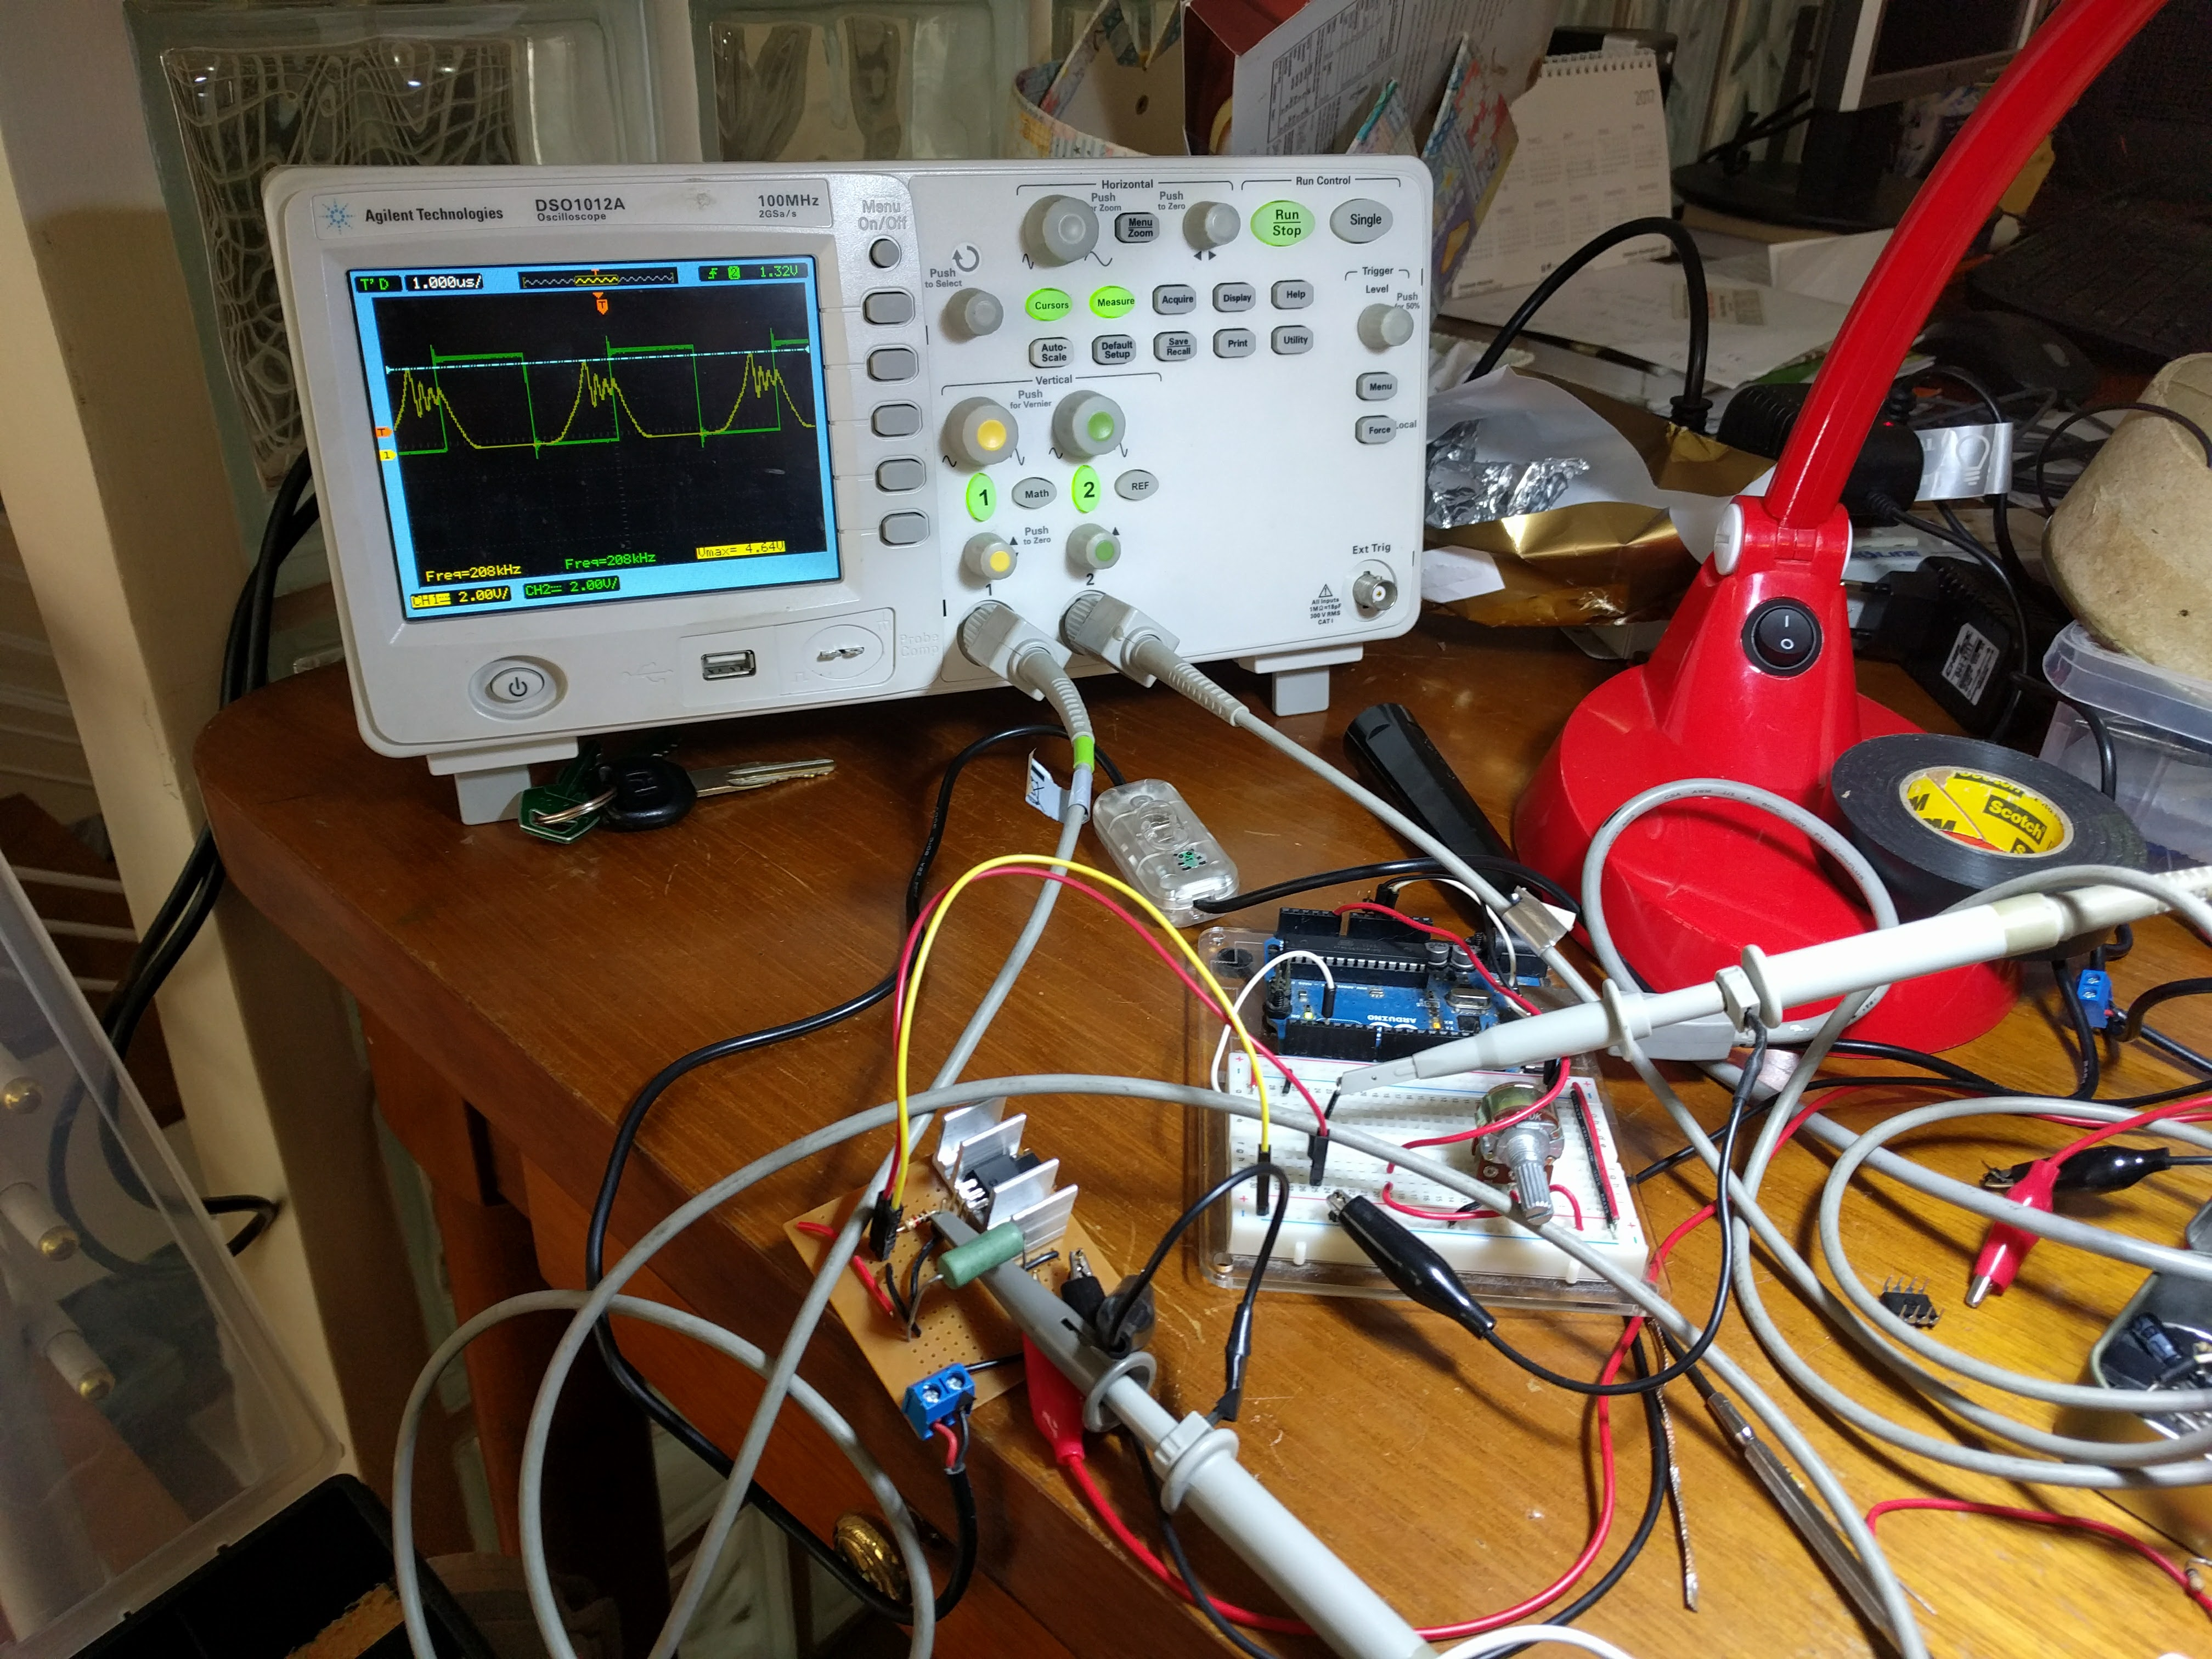
\includegraphics[width=0.5\textwidth, trim={22.5cm 69cm 87cm 16cm}, clip]{circuits/photos/TX_200k_without_filter.jpg}
		\legend{Fonte: Autores.}
	\end{figure}
	Nesse caso é muito mais evidente o amortecimento visto na onda. Atribui-se esse comportamento à componente capacitiva ao chavear o LED. No entanto, observa-se que não há \textit{feedback} do circuito na saída do gerador de funções, fato observado na última versão do circuito. O capacitor colocado adicionava um nível de complexidade desnecessário ao circuito, pois se carregava com oscilação da entrada. 
	
	Além disso, ele não preserva a forma de onda da entrada. Ainda é possível refinar mais a solução.
	
	\paragraph{Final - Filtro Passa-Altas}
	Por fim, realiza-se a correção dessa componente subamortecida utilizando um capacitor entre os terminais da \textit{source} do MOSFET e GND (observado em \autoref{fig_transmitter_lify_circuit_final}). 
	\begin{figure}[h!]
		\caption{\label{fig_transmitter_lify_circuit_final}Circuito final de transmissão de dados LiCy, utilizando um filtro passa-altas.}
		\centering
		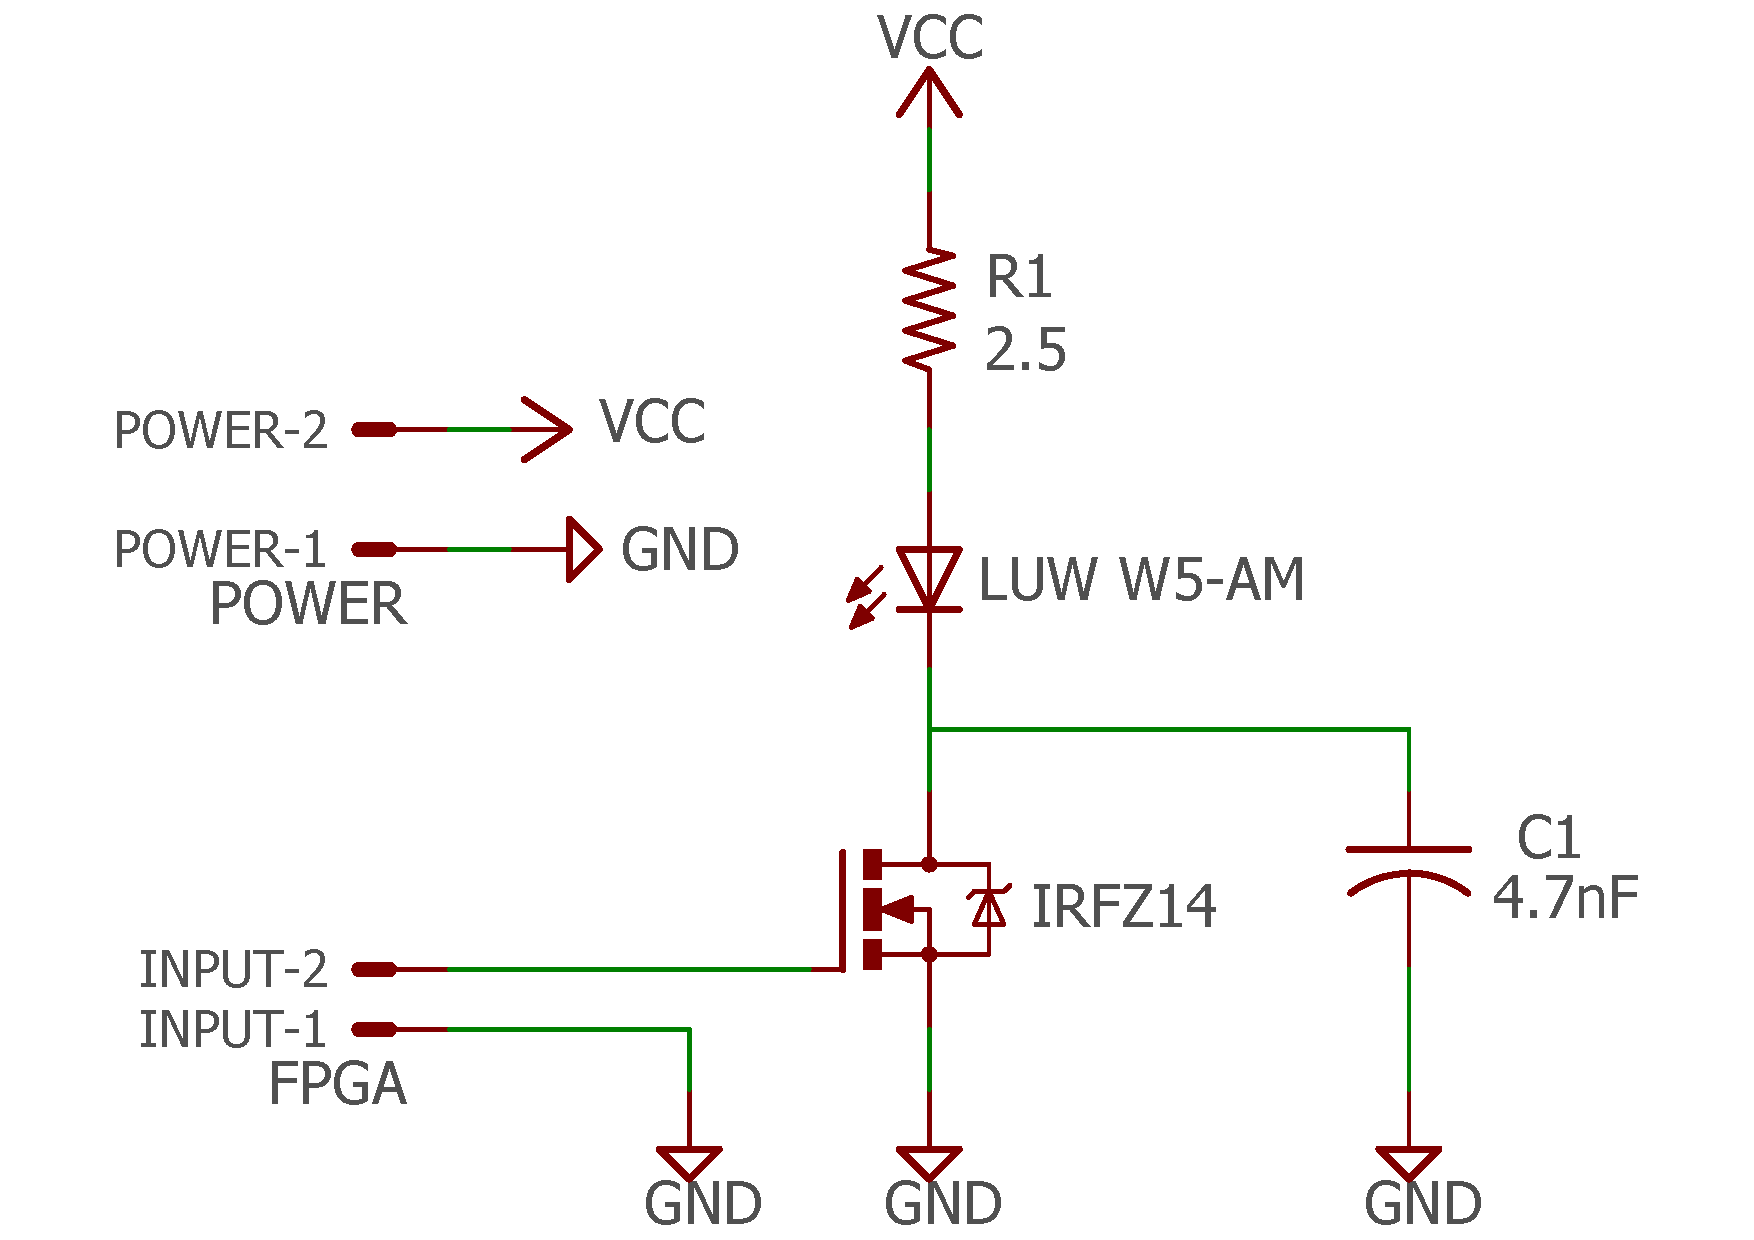
\includegraphics[width=0.6\textwidth, trim={2cm 0cm 2cm 0cm}, clip]{circuits/transmitter_lify.pdf}
		\legend{Fonte: Autores.}
	\end{figure}
	
	\begin{figure}[h!]
		\caption{\label{fig_transmitter_lify_circuit_final_r1} Forma de onda após adicionar um capacitor que age como filtro passa-altas. Está defasada em 180$\degree$. }
		\centering
		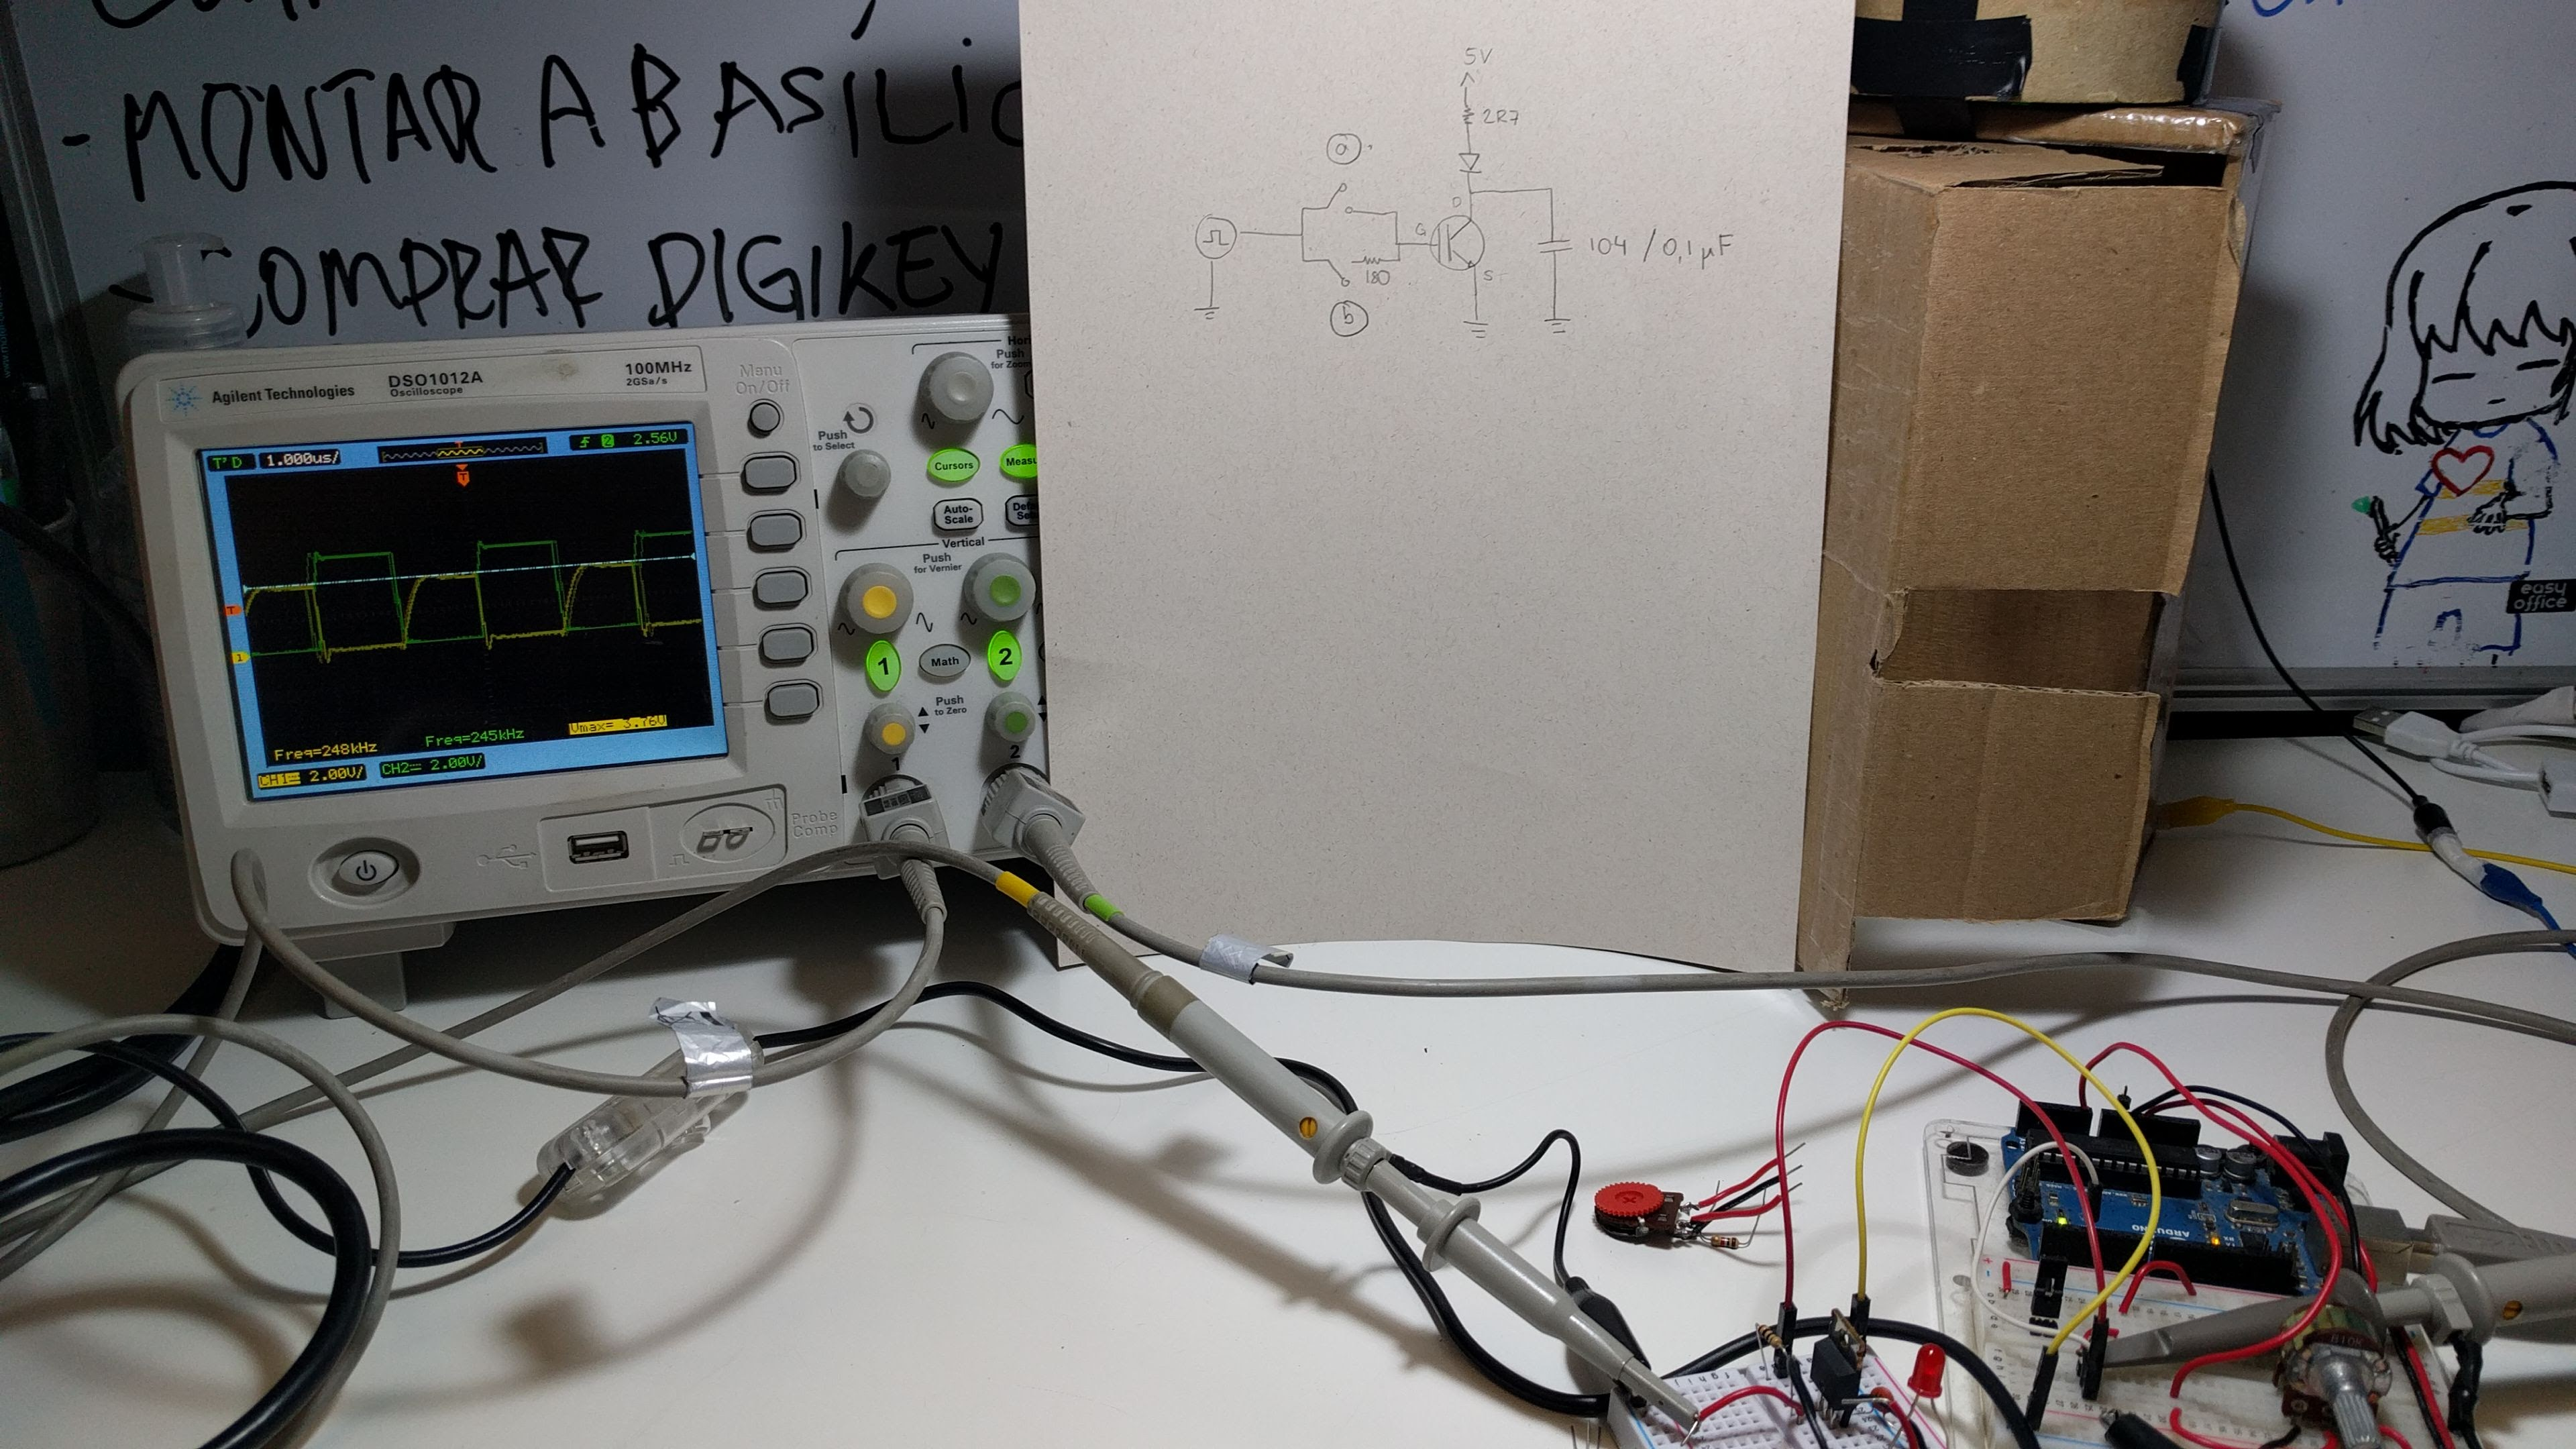
\includegraphics[width=0.5\textwidth, trim={5cm 30cm 90cm 20cm}, clip]{circuits/photos/TX_200k_with_filter.jpeg}
		\legend{Fonte: Autores}
	\end{figure}
	Esse capacitor atua como filtro passa-altas e remove a componente AC da saída para o LED. O comportamento não fica exatamente igual à entrada, mas é satisfatório, pois o período é muito similar, chaveando o LED corretamente. A forma de onda resultante pode ser observada na \autoref{fig_transmitter_lify_circuit_final_r1}. Está defasada em 180$\degree$.

	\subsection{Receptor}
	
	A recepção será feita utilizando os conceitos apresentados nas seções \ref{section:light-reception}, \ref{section:adc},  \ref{section:highpass-filter}, \ref{section:dc-bias} e \ref{section:band-filter}.
	
	\subsubsection{Recepção Luminosa}
	Para o recebimento luminoso, foi utilizado um circuito da "Application Notes" da \cite{datasheet-opa380}, simplificado e esquematizado na \autoref{fig_transimpedance_amp_complex_outer}, diferente do utilizado na Metodologia (\autoref{figure:transimpedance-amp-simple}). Com $V_{bias} = 2.5V$ polarizando reversamente o fotodiodo, uma resposta mais confiável era recebida pelo componente. O valor escolhido de R1 e R2 foram  1M$\Omega$ e 100k$\Omega$.
	
	\begin{figure}[htb]
		\caption{\label{fig_transimpedance_amp_complex_outer}Circuito e saída de um amplificador de impedâncias. No circuito, o fotodiodo é reversamente polarizado por $V_{bias}$. No osciloscópio, a saída está marcada em amarelo enquanto a saída do LED está em verde.}
		\begin{subfigure}{.5\textwidth}
			\centering
			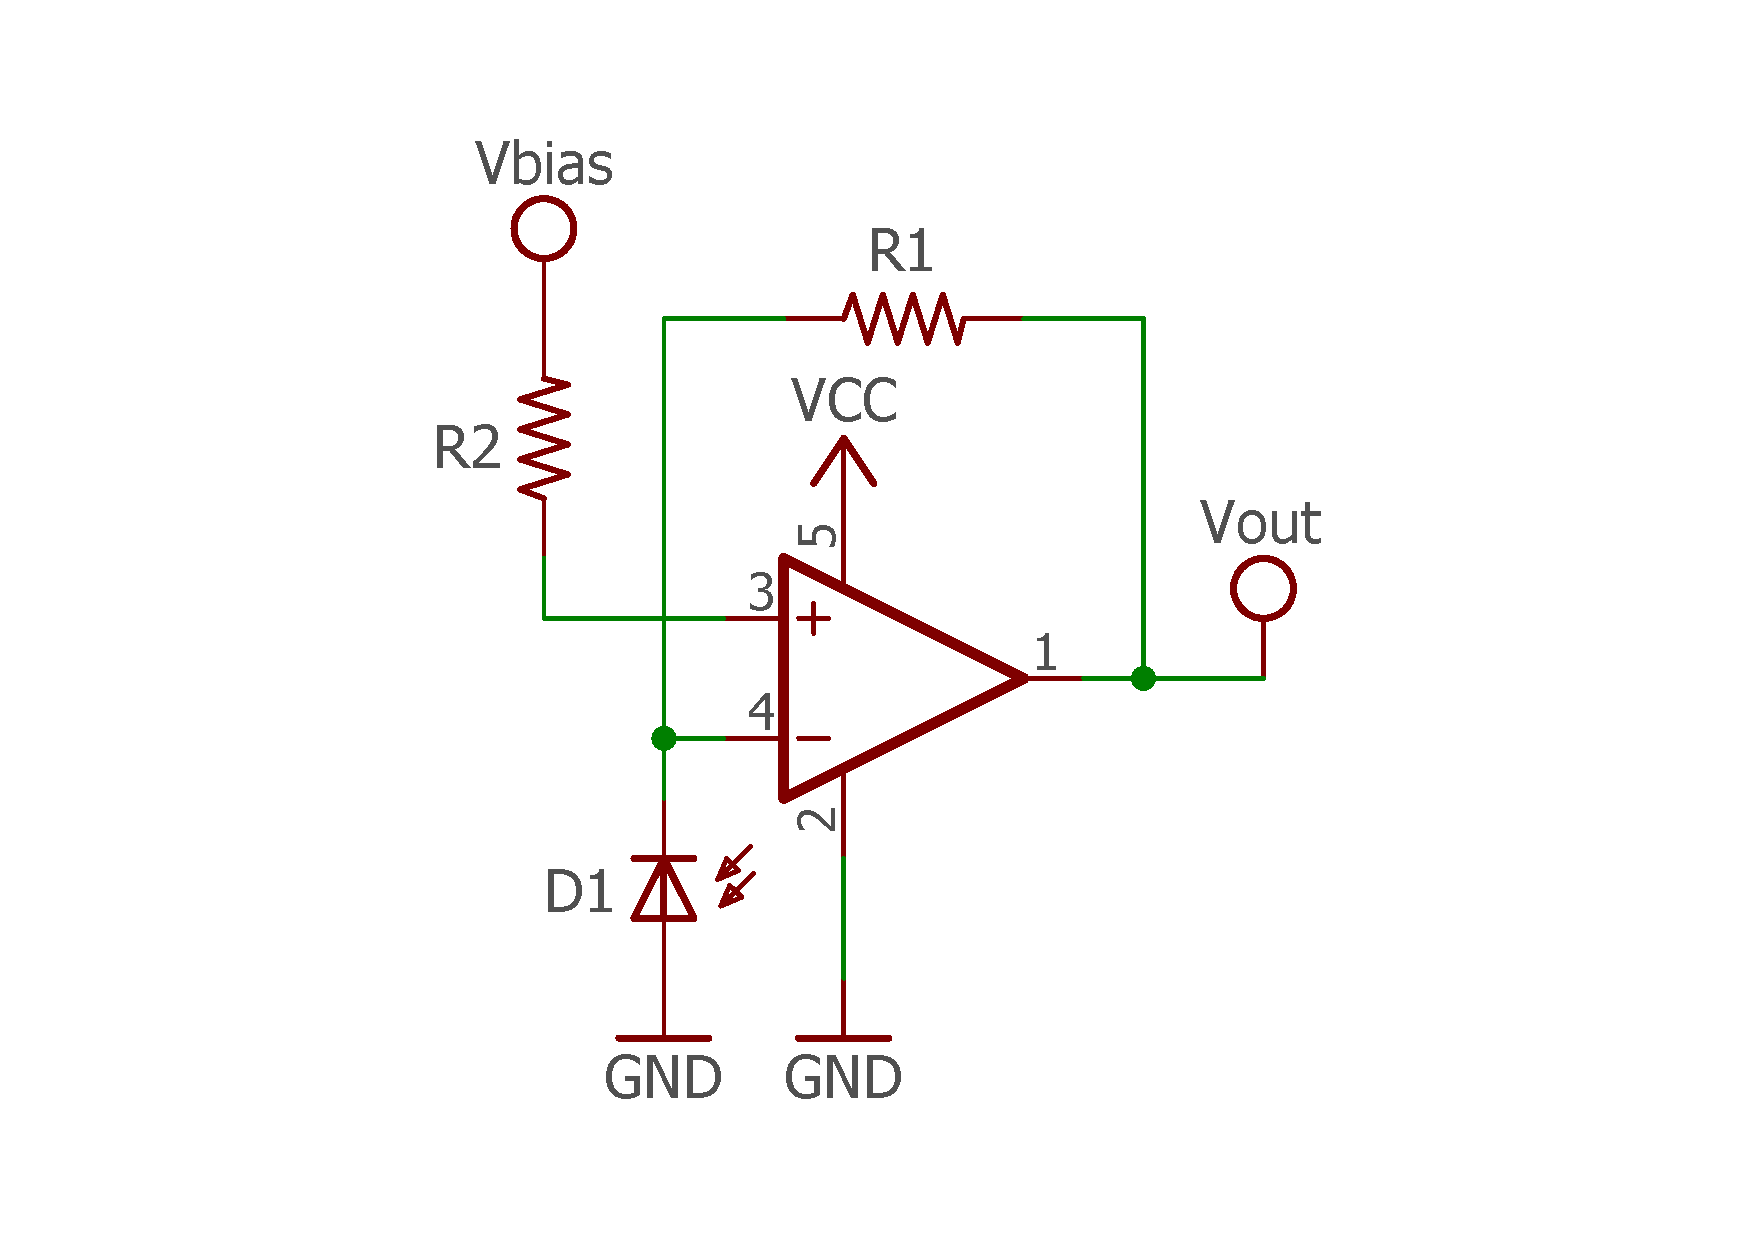
\includegraphics[width=1\textwidth, trim={1cm 1cm 1cm 2cm}, clip]{circuits/transimpedance_amp.pdf}
		\end{subfigure}
		\begin{subfigure}{.5\textwidth}
			\centering
			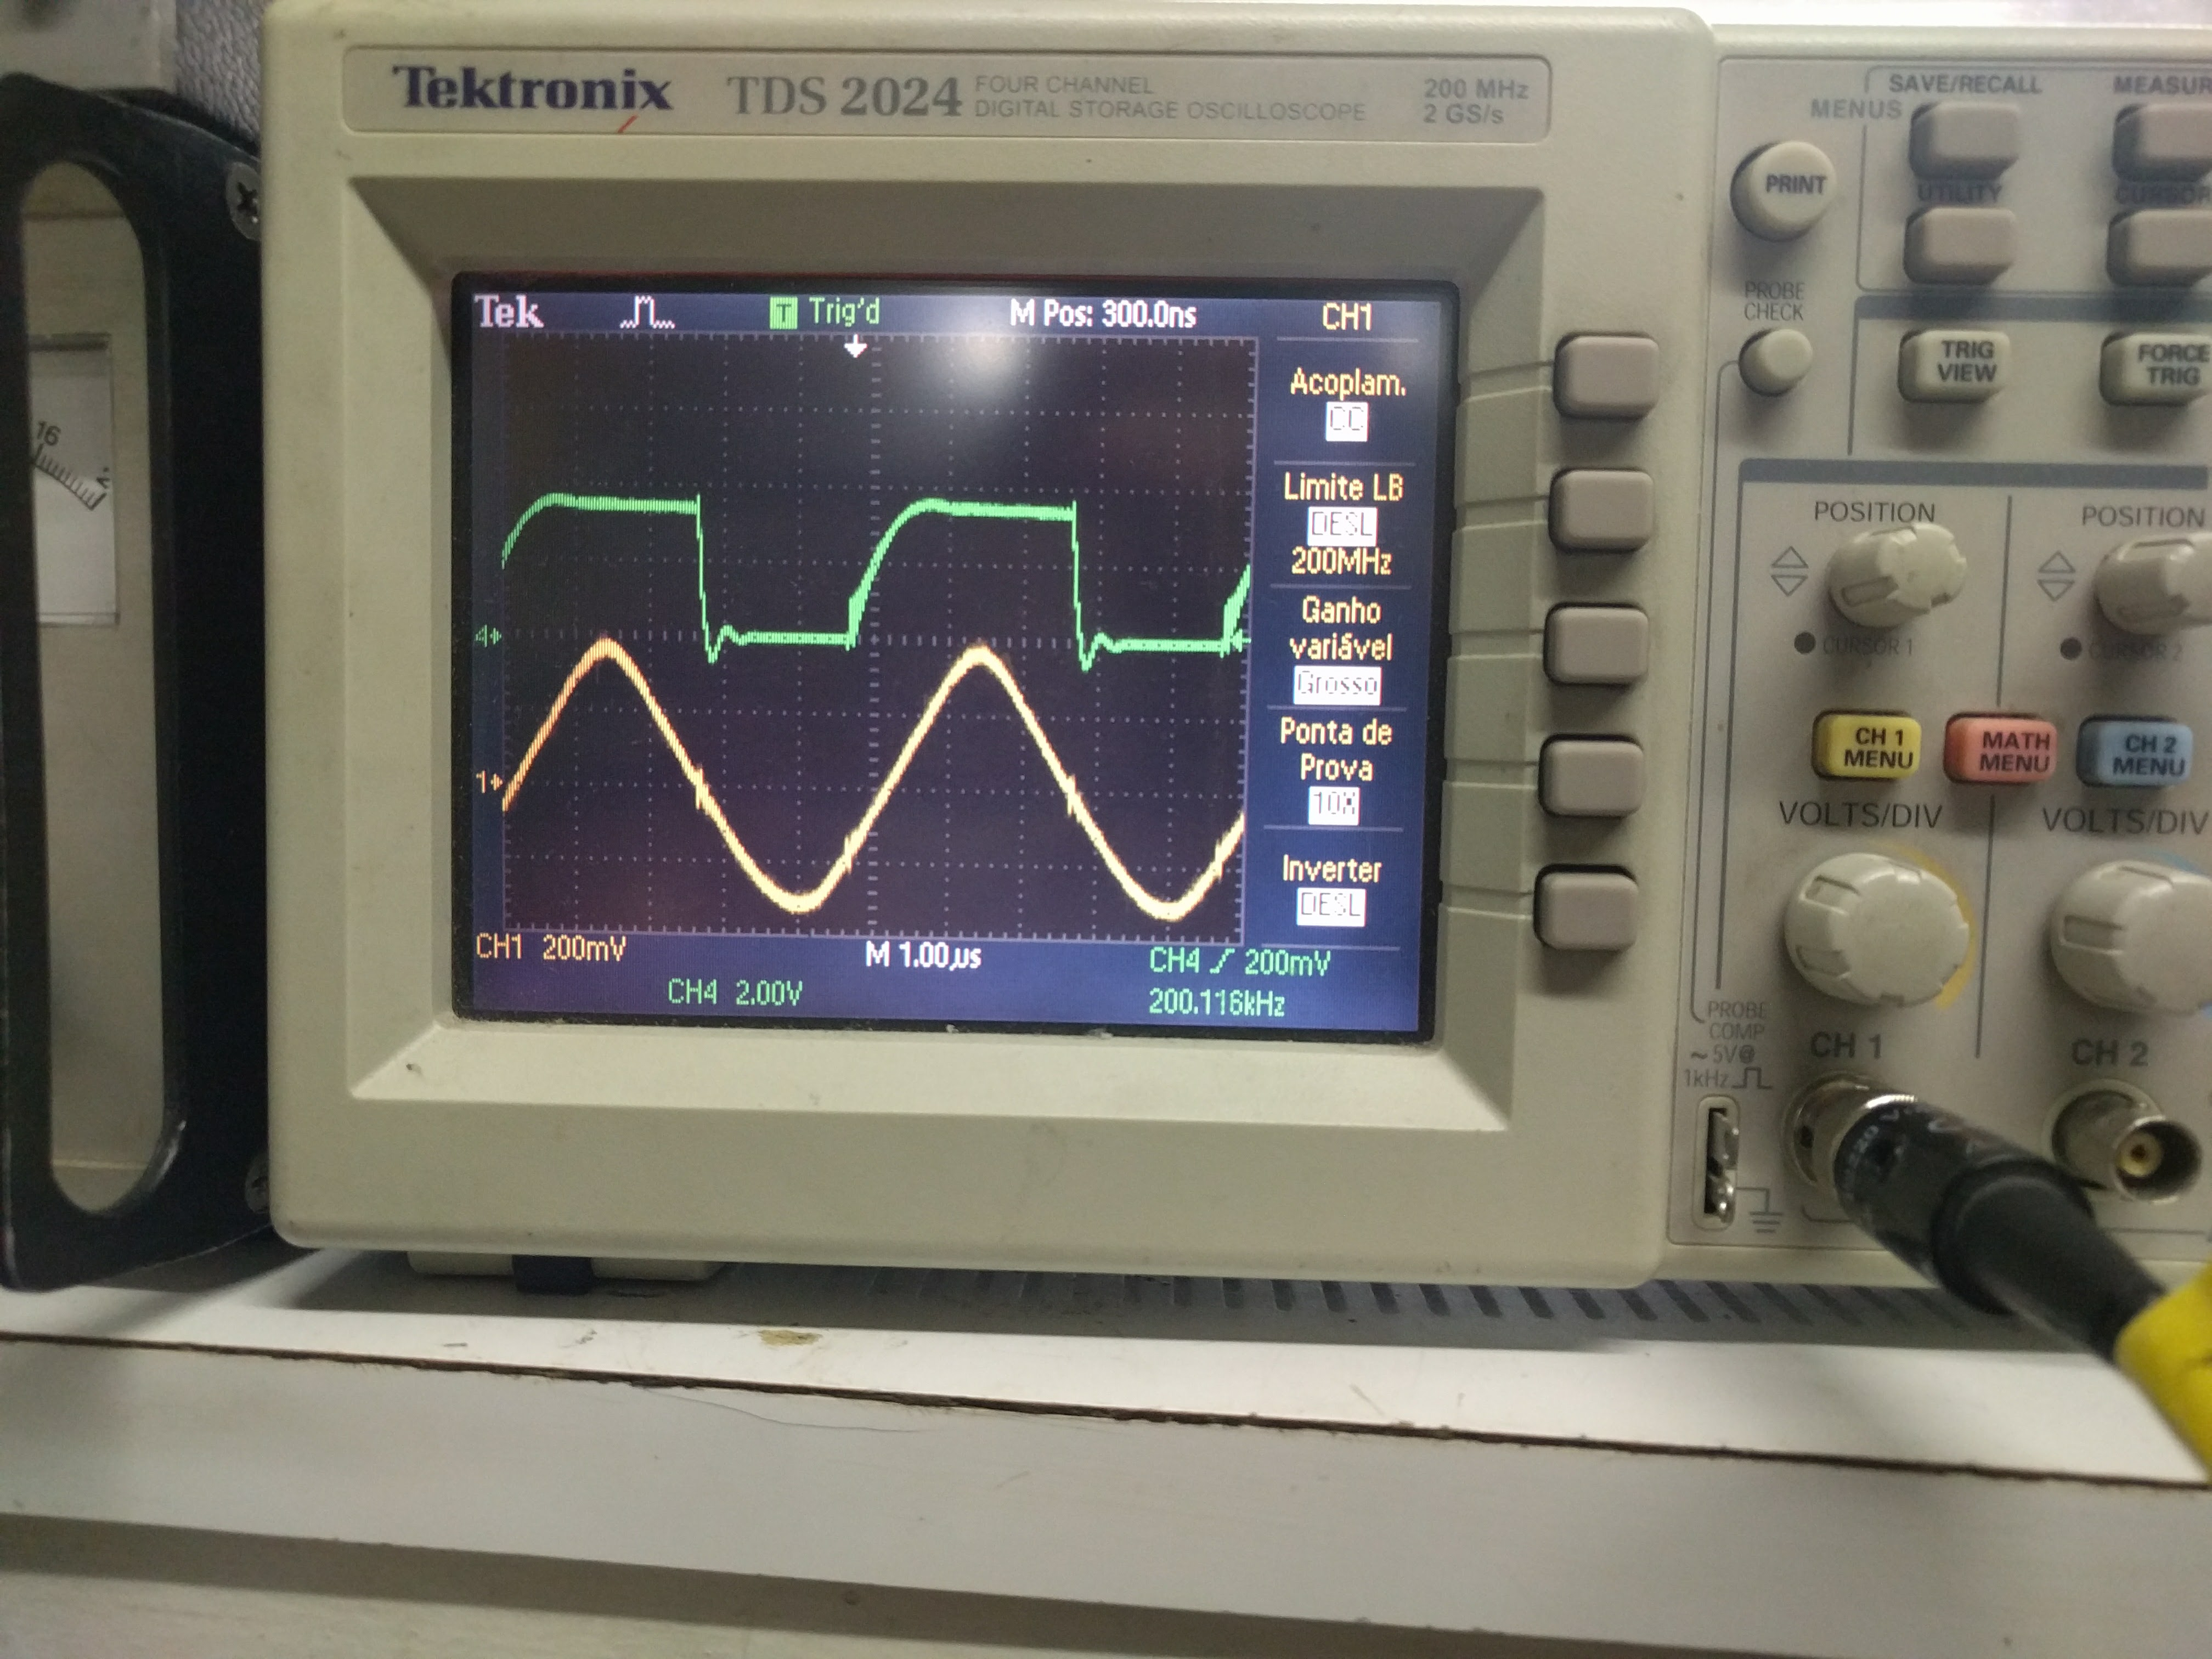
\includegraphics[width=1\textwidth, trim={25cm 35cm 40cm 15cm}, clip]{circuits/photos/RX_TIA_result.jpg}
		\end{subfigure}
		\legend{Fonte: Autores.}
	\end{figure}

	No osciloscópio, a componente DC da saída do amplificador de transimpedância é zero. No entanto, esse valor é apenas zero quando o padrão da oscilação luminosa se estabiliza. Entrando em detalhes: nesse e em todos casos de teste, o receptor está sendo submetido a uma onda quadrada de $f = 200kHz$. Como a norma define Manchester como código de RLL, é providenciado balanço DC ao receptor (são transmitidos a mesma quantidade de zeros e uns). Então o fotodiodo se desestabilizará quando há movimentação dos módulos ou quando há mudança na iluminação do ambiente.
	
	Para remover esses fatores de incerteza, o circuito de passas baixas com acomplamento DC $V_{ref} = 1V$ foi projetado a partir da \autoref{plot-post-bias1v}. Para obter uma voltagem de referência de 1V foi utilizado um divisor resistivo de 12k e 47k. 
	
	\begin{equation}
	V_{out} = V_{in} \cdot \frac{12k}{12k + 47k} = V_{in} \cdot \frac{12k}{59k} \approx \frac{V_{in}}{5} = \frac{V_{CC}}{5} \approx 1V
	\end{equation}
	
	\subsubsection{Conversor Analógico-Digital}
	
	Com a onda em $V_{DC} = 1V$, é possível utilizar o comparador definido na \autoref{fig_double_comparator} para converter a onda senoidal em uma onda quadrada, com níveis compatíveis com a FPGA.
	
	A voltagem de referência do comparador deve ser a mesma que a voltagem $V_{ref}$ do filtro passa-baixas, provenientes do divisor resistivo. O circuito final integrado do receptor pode é analisado na \autoref{fig_receiver_lify_circuit_final}.

	\begin{figure}[htb]
		\caption{\label{fig_receiver_lify_circuit_final}Circuito esquemático final de recepção de dados LiCy.}
		\centering
		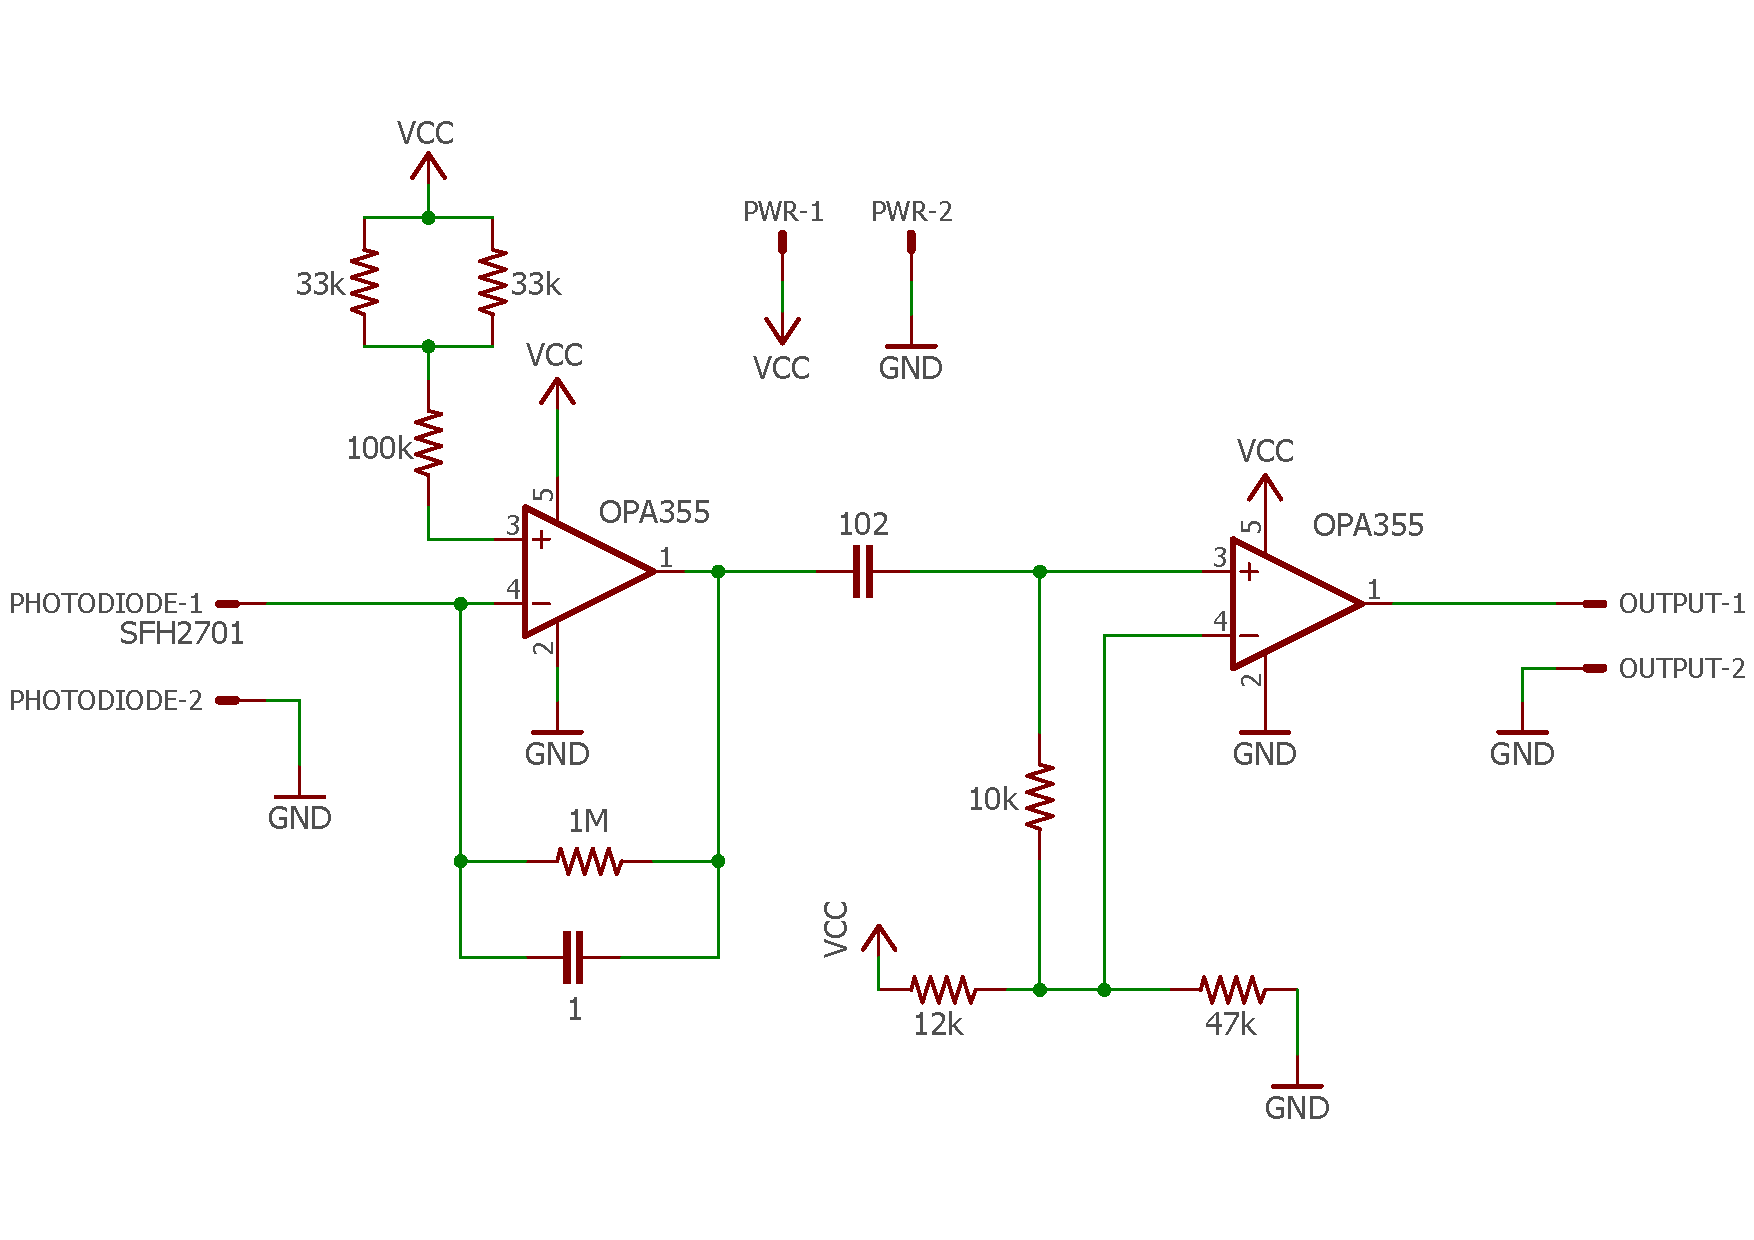
\includegraphics[width=0.7\textwidth, trim={0cm 1cm 0cm 1cm}, clip]{circuits/receiver_lify_final.pdf}
		\legend{Fonte: Autores.}
	\end{figure}
	
	Os testes realizados foram bem sucedidos e resultaram na onda da \autoref{fig_receiver_lify_circuit_final_r1}. Nela é possível observar a medição do período da onda resultante convertida, que foi 4.88us, muito próximo de 5us, período para 200kHz.
	
	\begin{figure}[htb]
		\caption{\label{fig_receiver_lify_circuit_final_r1}Saída do transmissor em verde e saída digital convertida do receptor em amarelo. É possível observar uma defasagem de 90$\degree$ em relação às ondas.}
		\centering
		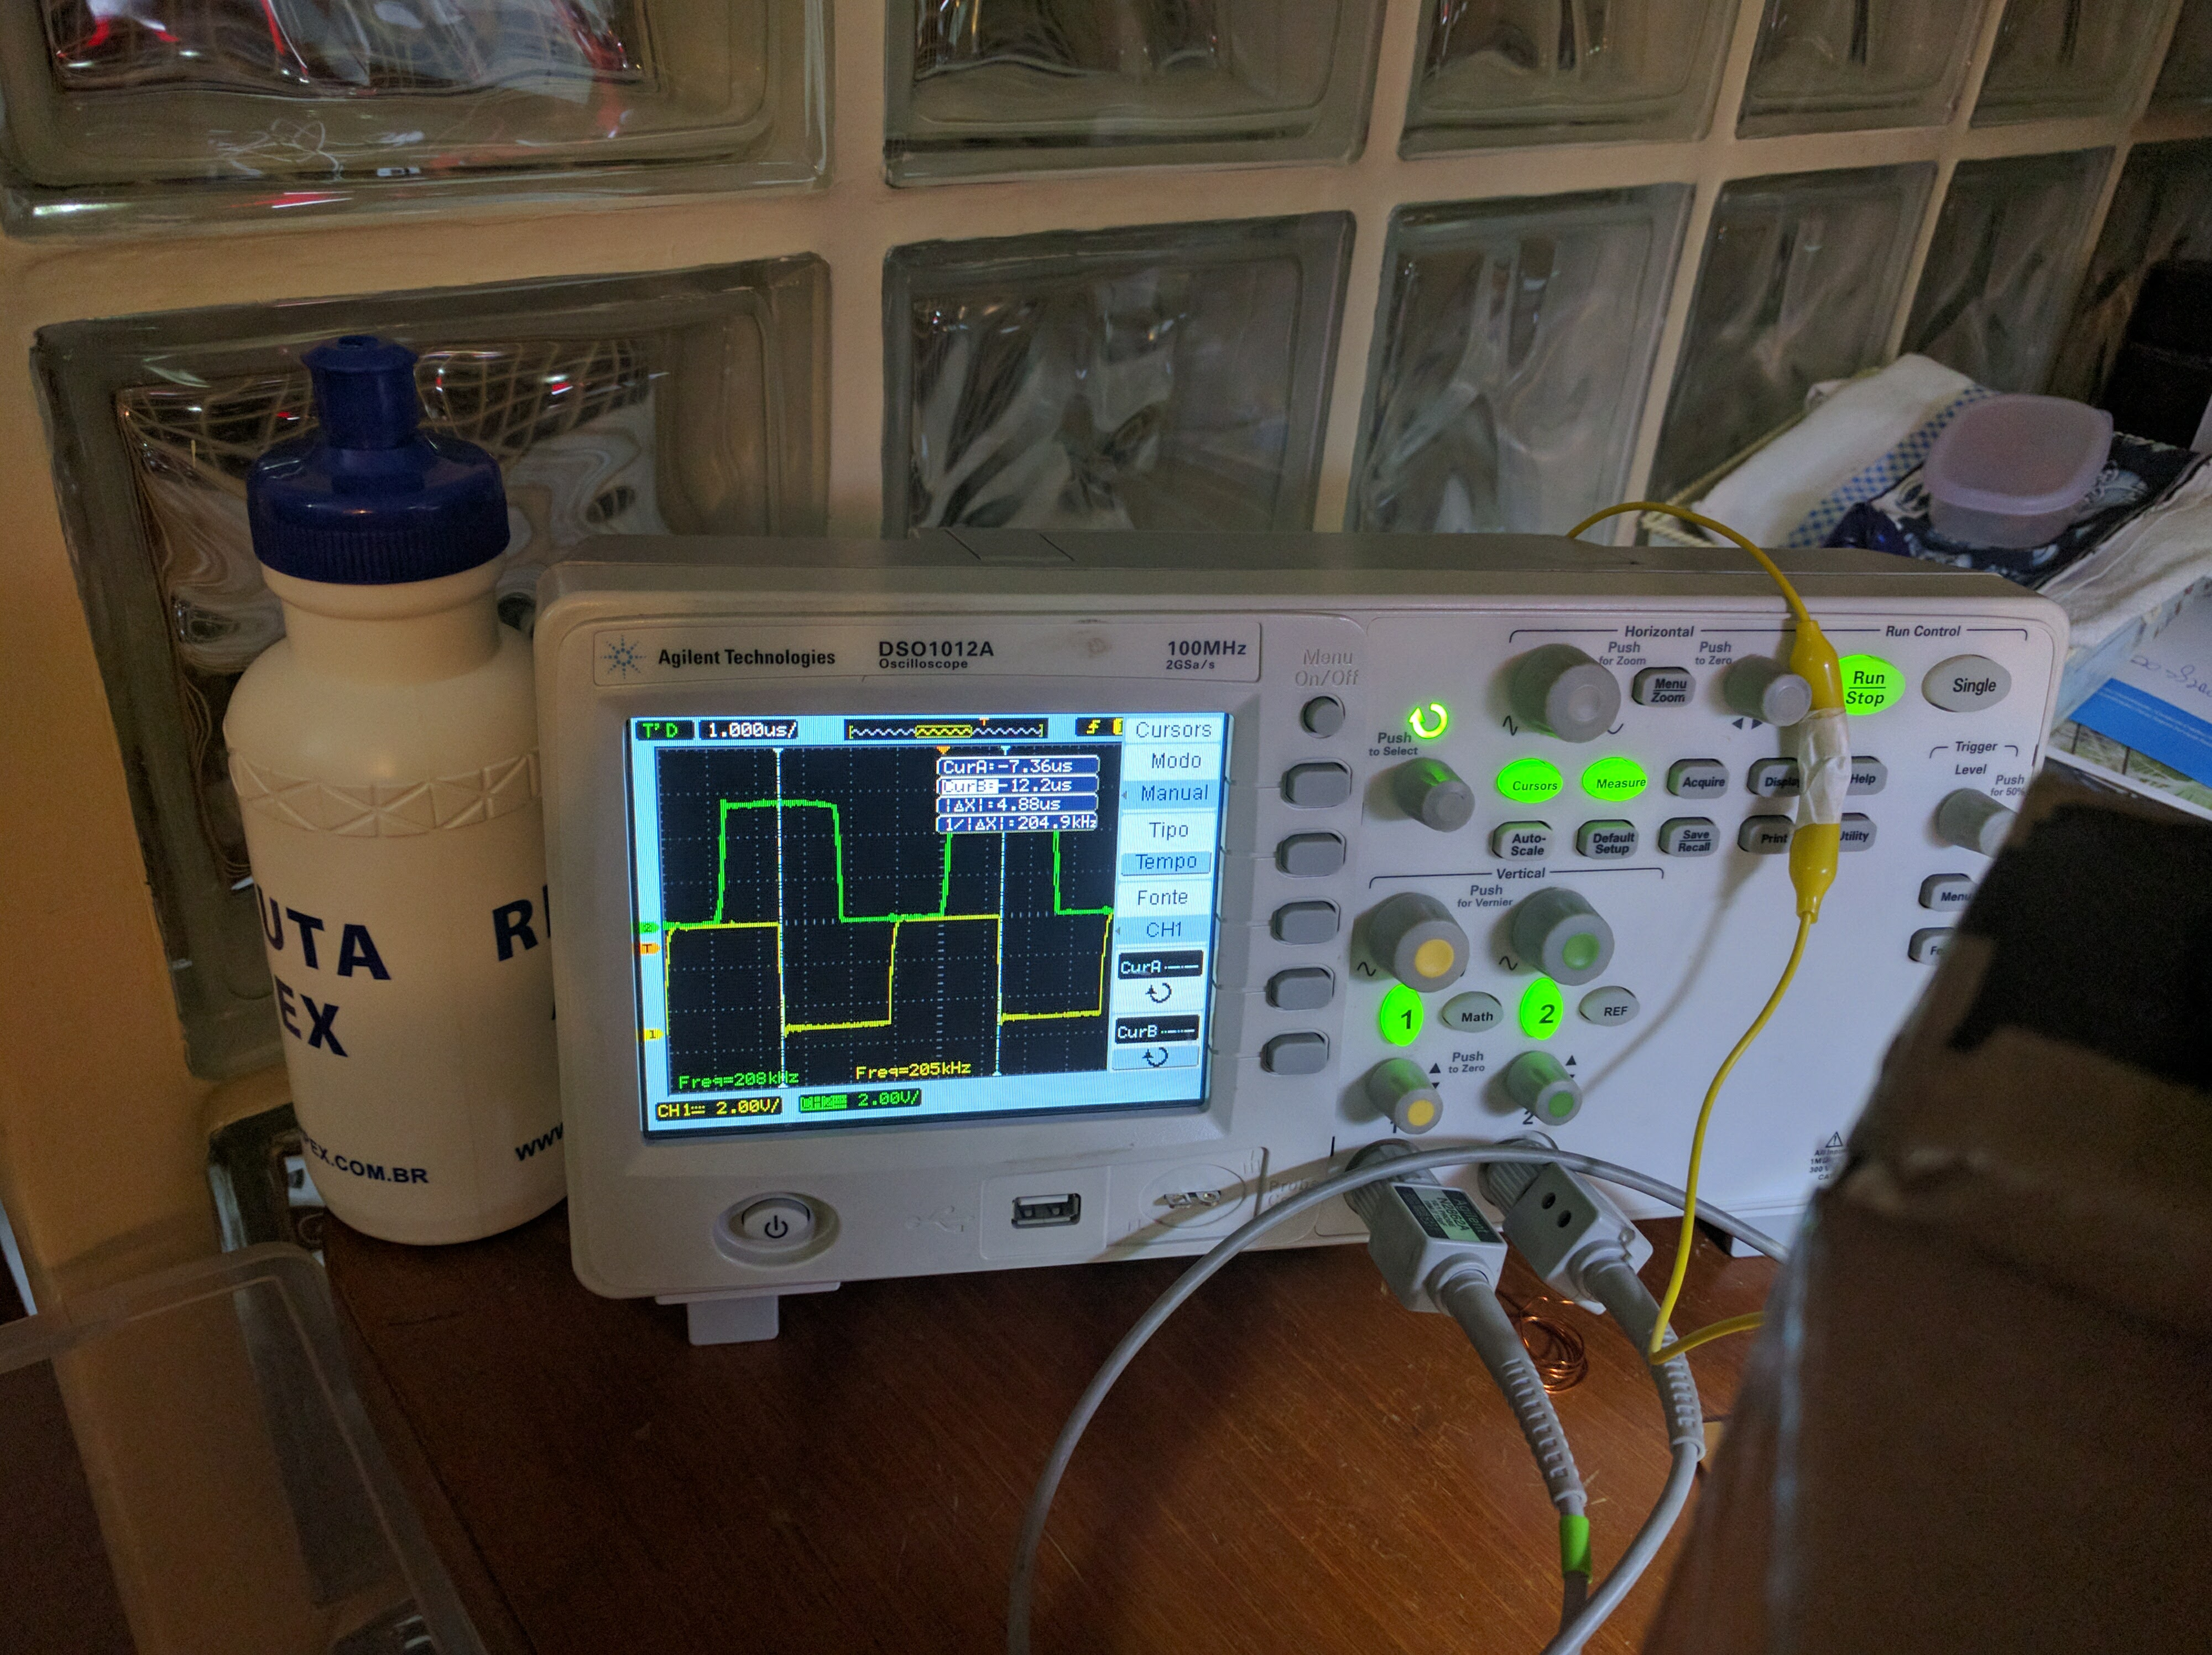
\includegraphics[width=0.7\textwidth, trim={36cm 30cm 60cm 40cm}, clip]{circuits/photos/TXRX_final_fixed.jpg}
		\legend{Fonte: Autores.}
	\end{figure}
	
	Em seguida será realizada a integração entre a parte analógica e digital do trabalho.
	
	\subsection{UART}
	
	UART, ou \textit{Universal Asynchronous Receiver/Transmitter} é o componente utilizado para fazer comunicação entre dispositivos. A transmissão de dados é feita a partir de pacotes compostos por: \textit{bit} de início, \textit{data frame}, \textit{bit} de paridade e \textit{bit} de fim.
	\begin{figure}[h]
		\caption{\label{figure:uart-frame}Quadro de mensagem da UART utilizada no projeto.}
		\centering
		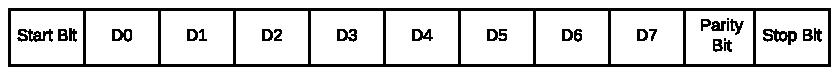
\includegraphics[width=0.9\textwidth]{uart/frame.pdf}
		\legend{Fonte: Autores.}
	\end{figure}
	
	Gerador de Baud: recebe um \textit{clock} de entrada e o divide para gerar o \textit{baud clock}. A frequência do \textit{baud clock} é dezesseis vezes o \textit{baud rate.} Quando a UART está recebendo o bit de entrada é amostrado no oitavo ciclo do baud clock para o esquema de \textit{oversampling} dezesseis vezes.
	
	\begin{figure}[h]
		\caption{\label{figure:uart-txrx}\textit{Oversampling} com \textit{baud clock}.}
		\centering
		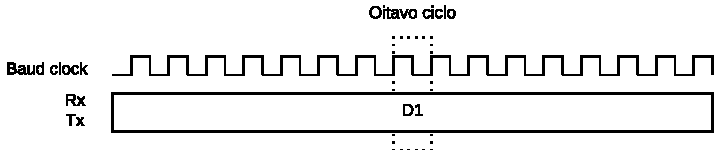
\includegraphics[width=0.9\textwidth]{uart/txrx.pdf}
		\legend{Fonte: Autores.}
	\end{figure}
	
	
	
	Receiver timing and control
	Transmitter Timing and control

	\section{Integração}
	
	\subsection{Etapas da Integração}
	O processo de integração seguiu o seguinte método: primeiro testaram-se unitariamente todos os componentes digitais. Uma vez concluídos os testes unitários feitos por meio de testbenches do Quartus, existiram duas frentes de integração: codificação e decodificação. Ambas são análogas, com exceção da presença do circuito de sincronização do módulo decodificador. É importante relatar que alguns subcomponentes foram testados unitariamente na própria FPGA, a fim de garantir que não houvesse comportamentos não previstos quando da integração. 
	
	O próximo passo da integração foi gravar o decodificador e o codificador na FPGA e testá-los separadamente. Neste caso, utilizou-se a ferramenta Signal Tap, onde se conecta a memória gravada a uma interface USB, controlam-se sinais de entrada e se observam as saídas. Uma vez que os testes foram satisfatórios, a integração de hardware digital pôde se concluir. Nesta última etapa, foram primeiro integrados codificador e decodificador dentro do próprio Quartus. Por fim, o circuito integrado foi gravado na FPGA, para mais testes, que antecederam os testes digitais finais, onde o transmissor e o receptor operaram cada um numa memória diferente, com clocks diferentes e um cabo como interface.
	
	Uma vez que se obteve os dois circuitos digitais principais operantes, cada um foi integrado com seu respectivo hardware analógico. Antes disso, o receptor e o transmissor analógico já haviam sido testados, com auxílio de uma fonte de sinais digitais na entrada do transmissor e um osciloscópio na saída do receptor.
	
	\subsection{Decisões tomadas na Integração}
	
	\section{Resultados}
	
